\chapter{Propagating the Uncertainty of Stereo Images}\label{chap:propagating}
This chapter details the work conducted on the propagation of uncertainty from images into the cost curves of dense matching problems. We consider a simple model of uncertainty on the input images, a dependency model between the uncertain intensities of the images, and estimate the resulting uncertainty on the output cost curves. This chapter takes up work and data already published \cite{malinowski_copulas_2022, malinowski_uncertainty_2023, malinowski_robust_2024}.

\section{Sources of uncertainty in stereo matching}\label{sec:sources_of_uncertainty}
\todoroman{Points à aborder: Atmospheric correction, vibration, resolution of a pixel, discretization.
CO3D mission will not have the epipolar line correction problem that is encountered with pleiades images.
Epipolar line rectification for Pléiades is a problem that is not dealt here.}

To maintain simplicity in this section, we will not consider panchromatic images, such as Pléiades products, encoding the reflectance values as positive integer, usually contained in $[0, 5000]$. Instead, we consider grayscale images that have intensity levels quantified within the range $[0, 255]$, which will represent our measurable space $\X$. We hypothesize that a pixel's intensity value can deviate by no more than $1$ level from its observed value, with the observed value being the most likely. This hypothesis arises from the noise of the sensor capturing the image, from pre-processing steps (see section \ref{sec:classical_stero_pipeline}) or from the quantification of observed radiometric values into integers. We assume this simple hypothesis to keep our explanation straightforward. Consequently, we model the uncertainty of each pixel $p\in I_L,I_R$ intensity with a possibility distribution $\pi$, centered around the observed intensity $i_p\in[0,255]$:
\begin{equation}
    \pi(i_p)=1,\quad \pi(i_p\pm1)=\alpha\,,
\end{equation}\label{eq:pixel_possibility}
with $\alpha \in [0,1]$. The $\pm$ indicates that both positive and negative values are considered. In our simulation, $\alpha = 0.3$ for pixels in the left image and $\alpha = 0.4$ for pixels in the right image. We use different values of $\alpha$ for the left and right images because the uncertainty model may vary between images due to differences in exposure, noise levels, or camera calibration. This model effectively states that we accept any probability distribution supported within $[i_p - 1, i_p + 1]$ where the probability measure $P$ satisfies $\{P(A) \leq \sup_{i \in A} \pi(i)\}$ as an acceptable model for our uncertainty. The mass distribution function $m_p$ associated to this credal set possesses two focal sets $a^p$:
\begin{eqnarray}
    &m_p(a^p_1=\opi i_p, i_p\cli)=1-\alpha\,\nonumber\\
    &m_p(a^p_2=\opi i_p-1, i_p + 1\cli)=\alpha\,\label{eq:pixel_mass}
\end{eqnarray}
with $\opi\cdot, \cdot\cli$ referring to integer intervals. In particular, $\opi i_p, i_p\cli$ correspond to the singleton $\{i_p\}$.

It is important to note that in this disparity estimation problem, we only account for the uncertainty in our input image intensities, without considering the uncertainty in our cost function's ability to correctly identify the true disparity as its minimum. In other words, we do not account for the uncertainty arising from the difference between ``two patches are very similar'' and ``the pixels at the center of the patches are homologous''. To better illustrate this, imagine a scenario where two pixels should be matched, but the surrounding patches are dissimilar. In this case, the cost function between those two patches would be high, potentially leading to the selection of a different patch with a lower cost function as the estimated disparity. The correct disparity would not be the minimum of the cost curve. This problem tends to appear more often when considering large windows, as the cost function can `average' the similarity of all its pixels, regardless of the similarity of the central ones. 

We consider the Sum of Absolute Differences (SAD) as our cost function, defined as follows. Given patches $W_L\subset I_L$ and $W_R\subset I_R$ of the same shape with $n$ pixels (usually squares):
\begin{align}
    \mathrm{SAD}(W_L, W_R) = \sum_{(p_i, q_i)\in (W_L, W_R)}|I_L(p_i) - I_R(q_i)|\label{eq:SAD}
\end{align}
where $p_i$ and $q_i$ are pixels at the same position $i$ in their patch. For convenience purposes, we will refer to the Absolute Difference as AD. This cost function is not ideal compared to more complex state-of-the-art cost function (\cite{zbontar_stereo_2016}, \cite{laga_survey_2022}), but it is preferred here to focus on simplicity and to ease didactic explanations regarding uncertainty propagation. An illustration of the SAD cost function can be found in Figure \ref{fig:SAD}. Furthermore, we will not consider in this chapter the use of Semi Global Matching (or similar regularization methods), as it necessitates many operations due to its recursive formulation and thus greatly increases complexity for the uncertainty propagation. We diverge from state-of-the-art methods to keep explanations as simple as possible, however the modeling of uncertainty for more advanced cost functions and SGM methods will be considered in chapter \ref{chap:epistemic_uncertainty}.

An ideal cost function would generate a cost curve with a unique minimum corresponding to the correct disparity. In practice, such a function is hard to determine. There is no guarantee that the minimum is unique, nor that it corresponds to the correct disparity. 

\begin{figure}
    \centering
    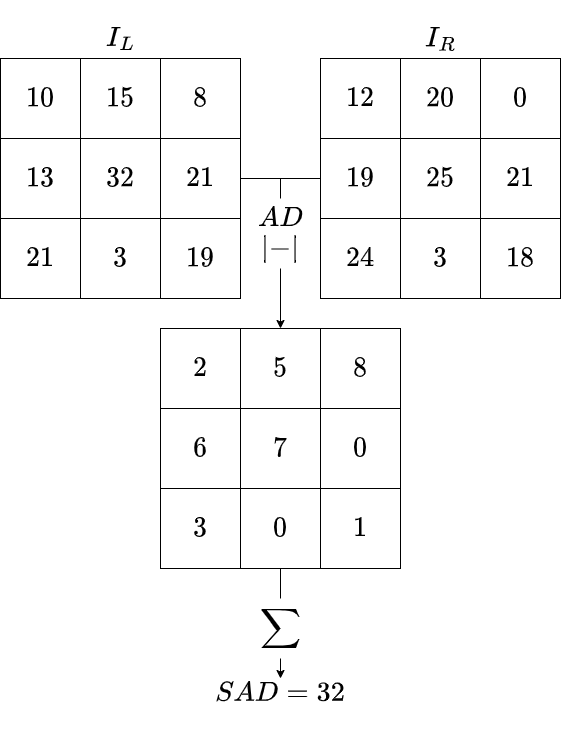
\includegraphics[width=0.5\linewidth]{Images/SAD.png}
    \caption{Diagram representing the $SAD$ cost function between two $3\times3$ patches.}
    \label{fig:SAD}
\end{figure}

We presented the uncertainty models for pixels in both images, but we also need to define the dependency model between every pixels of both images. In our case, we propose to model their dependency with the product copula if the pixels are not from the same physical object (meaning that the value of their intensities are independent), and by a Gaussian copula with a covariance matrix parameterized by a correlation matrix $R$. The correlation between the uncertain pixel intensities is based on a segmentation $S:(I_L\cup I_R)\rightarrow[\![0,K]\!]$, $K\in\mathbb{N}$, of the images, performed on the ground truth disparity of each pixel. Given two pixels $(p, q)\in(I_L\cup I_R)^2$, their covariance is determined by:
\begin{equation}
    \mathrm{cov}(p, q) =
    \begin{cases}
        1 &\text{ if }p=q\,,\\
        \rho_k, &\text{ if } p\ne q\text{ and }S(p)=S(q)\,, \\
        0, & \text{otherwise}\,.
    \end{cases}\label{eq:correlation}
\end{equation}
During the simulations, the segmentation contains $K=8$ different clusters, and for every $k$ in $[\![0,K]\!]$, $\rho_k$ is assigned an arbitrary value between $0.9$ and $1$.

We can thus build a correlation matrix $R$ for all pixels of $(I_L\cup I_R)$, and sample a perturbation on all of the pixels using a Gaussian copula with this correlation matrix. The Gaussian $18-$copula used to model the dependency between marginal masses in the uncertainty propagation step (using equation \eqref{eq:joint_mass}) is also constructed using Equation \eqref{eq:correlation}. 

\section{Propagation of the Uncertainty with Belief Functions}
This section will present how we can compute a Belief function on the matching cost curve values from the original beliefs as well as a copula representing the dependency between variables. We first detail how it can be done in the precise case, as the imprecise setting is similar. We use the case of the SAD cost function to illustrate the process.

First, let us present the propagation of uncertainty in the precise bivariate case. Let $f:\X_1\times\X_2\rightarrow\mathcal{Z}$ be a mapping and we define the random variables $Z$ as $Z=f(X,Y)$. 
When considering precise probabilities, the mass distribution $p_Z$ on atoms of $Z$ is:
\begin{align}
    \forall z\in\mathcal{Z}, p_Z(z)=\sum_{\substack{x_1,x_2\\z=f(x_1,x_2)}}p(x_1,x_2).
\end{align}

Determining every $(x,y)$, whose image by $f$ equals $z$, is not always trivial. This becomes even more complex when we are considering copulas with $n>2$ variables. Note that the joint probability $p(x_1,x_2)$ is computed using a H-volume, which is the sum of $2^n$ terms, also increasing exponentially with the dimension. In the continuous case, the H-volume is replaced with the density $h$ of the joint CDF. The density of $Z$ is thus:
\begin{align}
    p_Z(z) = \int_{\X_1}\int_{\X_2}h(x_1,x_2)\mathds{1}(f(x_1,x_2)=z)dx_1dx_2,
\end{align}
Here, $\mathds{1}$ refers to the characteristic function.

Similarly, belief functions can be propagated by replacing the mass on atoms with the mass associated to the joint belief function. Given the joint mass distribution function $m_\times$ constructed with a copula as in equation \eqref{eq:joint_mass}, it is possible to compute the mass distribution function $m_Z$ of a random set $Z$ from $n$ marginal random sets:
\begin{align}
    \forall a^Z\subseteq\mathcal{Z}, m_Z(a^Z) = \sum_{\substack{a^1_i, \dots, a^n_j\\a^Z=f(a^n_1,\dots, a^n_j)}}m_\times(a^1_i, \dots, a^n_j)\label{eq:mass_propagated}
\end{align}
Computing the image of $f$ for every pair of focal sets $(a^1_i, \dots, a^n_j)$ is even more difficult than in the precise case, as we are computing reverse images of sets instead of real numbers. Propagation of uncertainty with a copula has also been investigated in the case of necessity functions in \cite{gray_dependent_2021}. To illustrate how to propagate the uncertainty using belief functions and a copula, we will use the SAD cost function as an example.

The SAD is used to compute the similarity between $3\times3$ windows $W_L, W_R$. We use the mass distribution $m_p$ of Equation \eqref{eq:pixel_mass} to represent the uncertainty of each pixel $p$. For every pair of pixels $p\in I_L, q\in I_R$, we note $\mathrm{AD}_{pq}=|i_p - i_q|$. There exists $3$ focal sets related to the absolute difference:
\begin{itemize}
    \item $a^{\mathrm{AD}}_1$ is the image of the AD of $a^p_1$ and $a^q_1$
    \item $a^{\mathrm{AD}}_2$ is the image of the AD of $a^p_2$ and $a^q_1$ or $a^p_1$ and $a^q_2$
    \item  $a^{\mathrm{AD}}_3$ is the image of the AD of $a^p_2$ and $a^q_2$
\end{itemize}
The non-monotonicity of the absolute value around $0$ needs to be taken into account to compute their exact image through the AD:
\begin{align*}
    a^{\mathrm{AD}}_1&=\opi\mathrm{AD}_{pq},~\mathrm{AD}_{pq}\cli\,,\\
    a^{\mathrm{AD}}_2&=\opi\mathrm{AD}_{pq} - 1,~\mathrm{AD}_{pq} + 1\cli\text{ if }\mathrm{AD}_{pq}>0\,,\\
            &=\opi\mathrm{AD}_{pq},~\mathrm{AD}_{pq} + 1\cli\text{ otherwise }\,,\\
    a^{\mathrm{AD}}_3&=\opi\mathrm{AD}_{pq} - 2,~\mathrm{AD}_{pq} + 2\cli\text{ if }\mathrm{AD}_{pq}>1\,,\\
            &=\opi\mathrm{AD}_{pq} - 1,~\mathrm{AD}_{pq} + 2\cli\text{ if }\mathrm{AD}_{pq}=1\,,\\
            &=\opi\mathrm{AD}_{pq},~\mathrm{AD}_{pq} + 2\cli\text{ otherwise}\,.
\end{align*}

Bounds of the AD are then summed to obtain the final values of the SAD focal sets. The mass $m_{\mathrm{SAD}}$ of those focal sets are computed using equations \eqref{eq:joint_mass} and \eqref{eq:mass_propagated}. To represent the dependency between pixels of both windows, a Gaussian $18$-copula is used. Splitting the problem using lower dimension copulas is tempting, similarly to what can be done with vine copulas (\cite{czado_vine_2022}). However this is a complex problem that will not be explored in this thesis. We will instead work with Gaussian copulas, introducing a simple method for creating a correlation matrix. This will also allow us to present simple optimisation to reduce computation complexity and splitting the copulas into mutually independent groups of variables. 

\section{Leveraging specificities to accelerate computations}
\todoroman{H Volume etc for SAD example, see IJAR.}

Determining the bounds of the SAD focal sets is mostly straightforward. However, computing the joint mass over two $3 \times 3$ windows is significantly more complex. For each combination of marginal focal sets, the mass $m_{\mathrm{SAD}}$ is computed using the $H$-volume of an $18$-copula, involving a sum of $2^{18}$ terms. Given that the uncertainty for each pixel is represented by $2$ focal sets, we need to evaluate $2^{18}$ combinations of these focal sets in total. This computation can thus become quite costly in memory and computation time, especially when computing it over a whole image. A strategy to reduce computation time is to leverage the fact that the focal sets derived from a possibility distribution (or equivalently from its necessity measure) form a nested family of sets. For simplicity, the following observations will be detailed in the case where there are $n=2$ sources of uncertainty to join, but they hold for every $n\geqslant2$. Propagating two necessity measures $\mathrm{Nec}_1:2^{\X_1} \rightarrow [0,1]$ and $\mathrm{Nec}_2: 2^{\X_2} \rightarrow [0,1]$ through a mapping $f: \X_1 \times \X_2 \rightarrow \mathcal{Z}$ using a copula $C$ does not generally result in a necessity measure, but rather a belief function.

For the special case where:
\begin{itemize}
    \item $\mathrm{Nec}_1$ and $\mathrm{Nec}_2$ are defined by symmetric uni-modal possibility distributions (typically triangular possibilities)
    \item $f$ is a monotone function applied to a linear combination $\alpha X_1 + \beta X_2 + \gamma$, with $(\alpha, \beta, \gamma) \in \mathbb{R}^3$
\end{itemize}
then the focal sets of $\mathrm{Nec}_{X_1}$ and $\mathrm{Nec}_{X_2}$ are families of nested sets that can be represented as:
\begin{align*}
    [\overline{X}_1-\delta x^1_i, \overline{X}_1+\delta x^1_i]\quad[\overline{X}_2-\delta x^2_j, \overline{X}_2+\delta x^2_j]
\end{align*}
with $\overline{X}_1\in\X_1,~\overline{X}_2\in\X_2$ and $\delta x^1_i,~\delta x^2_j$ positive scalars. This results in the focal sets $a_{ij}$ of $Z = f(X_1, X_2)$ having the following expression:
\begin{align*}
    a_{ij} = \left[ \alpha \overline{X_1} + \beta \overline{X_2} + \gamma - (|\alpha| \Delta x^1_i + |\beta| \Delta x^2_j), \right. \\
                 \left. \alpha \overline{X_1} + \beta \overline{X_2} + \gamma + (|\alpha| \Delta x^1_i + |\beta| \Delta x^2_j) \right],
\end{align*}
Those focal sets form a nested family of sets, which is a characteristic of necessity measures \cite{shafer_mathematical_1976}. When a monotone function is applied to these focal sets, the nesting property is maintained, although the symmetry of the sets might be lost. This implies that $\mathrm{Bel}_Z$ (the belief function derived from $Z$) behaves as a necessity measure under these conditions.

On the other hand, for more sophisticated functions, such as multiplication, exponential functions, or sigmoid functions, the nesting property might not hold. It's often easy to find counterexamples where the nested nature of the focal sets is disrupted when such functions are applied. The upcoming example illustrates this situation.

\begin{example}
    Consider the function $f(x_1,x_2)=(x_1^2+1)+(x_2^2+1)$, and the following marginal mass functions $m_1$ and $m_2$:
\begin{align*}
    &m_{1}([0]) = m^{1}_1>0,\, &m_{2}([1]) = m^{2}_1>0\,,\\
    &m_{1}([-2,2]) = m^{1}_2>0,\, &m_{2}([0,2]) = m^{2}_2>0\,.
\end{align*}
After propagating through the function $f$ with a copula $C$, one gets the joint mass $m_\times$:
\begin{eqnarray*}
    m_\times(f([0],[1])) =& m_\times([3]) &= C(m^{X_1}_1,m^{X_2}_1)\,,\\
    m_\times(f([-2,2],[1])) =& m_\times([3,7]) &= m^{X_2}_1 - C(m^{X_1}_1,m^{X_2}_1)\,,\\
    m_\times(f([0],[0,2])) =& m_\times([2,6]) &= m^{X_1}_1 - C(m^{X_1}_1,m^{X_2}_1)\,,\\
    m_\times(f([-2,2],[0,2])) =& m_\times([2,10]) &= 1 - m^{X_1}_1 - m^{X_2}_1 + C(m^{X_1}_1,m^{X_2}_1)\,.
\end{eqnarray*}
For most copulas and mass functions (for instance $C=C_\Pi$, and $m^1_1=m^1_2=m^2_1=m^2_2=m^1_1=0.5$), the output focal sets of $m_\times$ do not form a nested family, and thus defines a belief function that is not a necessity function.
\end{example}

The nesting property for uni-modal symmetric possibilities and monotone functions can be leveraged to streamline the computation of the bounds and masses of focal sets, particularly when all (AD) exceed $2$. This condition helps to circumvent the complications arising from the non-monotonic behavior of the absolute value function near $0$.

In the scenario where the focal sets are nested, we can use equation \eqref{eq:sklar_on_necessity} to compute the belief of any focal sets $a^1_i$ and $a^2_j$ associated with the necessity functions $\mathrm{Nec}_1$ and $\mathrm{Nec}_2$ respectively. For any copula $C$ it holds that:
\begin{align*}
    \mathrm{Bel}_\times(a^1_i, a^2_j) = C(\mathrm{Nec}_1(a^1_i),~\mathrm{Nec}_2(a^2_j))
\end{align*}

This implies that the joint belief function $\mathrm{Bel}_\times$ can be efficiently derived using only the marginal necessity functions $\mathrm{Nec}_X$ and $\mathrm{Nec}_Y$ along with the copula. Consequently, there is no requirement to calculate the joint mass directly, thereby eliminating the need to evaluate the $H$-volume as described by equation \eqref{eq:hvolume}. This means that the belief of every cylindrical event can be computed easily, with a single evaluation of a copula (contrary to what is required when using the H-volume). Computing the plausibility $\mathrm{Pl}_\times$ of cylindrical events $A_1\times A_2\subseteq\X_1\times\X_2$ is also straightforward by noticing that:
\begin{align*}
    \mathrm{Pl}_\times(A_1\times A_2) =& 1-\mathrm{Bel}_\times\left((A_1\times A_2)^c\right)\\
    =& 1 - \sum_{a_1\times a_2\subseteq(A_1\times A_2)^c}m_\times(a_1,a_2)\\
    =& 1 - (~\sum_{a_1\times a_2\subseteq A_1^c\times \X_2}m_\times(a_1,a_2) + \sum_{a_1\times a_2\subseteq \X_1\times A_2^c}m_\times(a_1,a_2) \\
    &- \sum_{a_1\times a_2\subseteq A_1^c\times A_2^c}m_\times(a_1,a_2) ~)\\
    =& 1 - \mathrm{Bel}_1(A_1^c) - \mathrm{Bel}_2(A_2^c) + \mathrm{Bel}_\times(A_1^c\times A_2^c)
\end{align*}
For events that are not cylindrical, then we need to compute the joint mass, either with the H-volume or using the fact that (\cite{shafer_mathematical_1976}):
\begin{align}
    \forall A\subseteq\X,~m_\times(A)=\sum_{a\subseteq A}(-1)^{|A/a|}\mathrm{Bel}_\times(A)\label{eq:bel_to_mass}
\end{align}

Another issue arises when computing the joint belief $\mathrm{Bel}_\times$ is that evaluating the copula for a high number of variables can become computationally heavy. This is the case for copulas for which only a closed form of its density is known, such as the family of Gaussian copulas. In that case, each evaluation necessitates integrating an $n$-variate function, leading to significant computational expense.

In our experiments, we processed images of size $375 \times 450$ with a disparity range of $[-60, 0]$. This resulted in the computation of over $10^7$ belief functions. Each belief function integrates the uncertainty from $2 \times 3 \times 3 = 18$ pixels, each having $2$ distinct focal sets. Consequently, we must compute the integral of more than $10^7 \times 2 ^{18}$ $18$-variate functions if we want to completely determine $\mathrm{Bel}_\times$, which is extremely time-consuming, even with optimized parallel processing. In practice, the number of evaluations is smaller as some combinations of marginal focal sets lead to the same propagated focal set. Nevertheless, calculating an $18$-dimensional Gaussian copula takes approximately $20$ seconds on an AMD EPYC $7713$ $64$-Core Processor at $2$ GHz, using Python and the SciPy library. However, we can significantly reduce the computation time by exploiting specific properties of our models and the copula.

Indeed, if the variables can be divided into multiple mutually independent sets of variables, the evaluation of the copula or of the H-volume is reduced. For instance, suppose that we can split the $n$ variables into two mutually independent sets $\{X_1,\dots,X_k\}$ and $\{X_{k+1},\dots,X_n\}$ with $k\in\opi1,n-1\cli$. Let $F_1,\dots, F_n$ be their marginals CDF. Then it holds that there exists a $k$-copula $C'$ and a $(n-k)$-copula $C''$ such that:
\begin{align*}
    &\forall (x_1,\dots,x_n)\in\X_1\tdt\X_n,\\
    &C(F_1(x_1),\dots,F_n(x_n))=C'(F_1(x_1),\dots, F_k(x_k))\cdot C''(F_{k+1}(x_{k+1}),\dots,F_n(x_n))
\end{align*}
which uses the same composition as vine copulas \cite{czado_vine_2022}, where the pair copula is the product copula. Knowing other types of dependency would allow to express the $n$-copula in terms of multiple lower dimension copulas, but the nature of our problem do not permit us to know such dependencies. 

\begin{remark}
    If a $n$-copula $C$ can be expressed as the product of a $k$-copula $C'$ and a $(n-k)$-copula $C''$, then the H-volume of $C$ is the product of the H-volume of $H'$ of $C'$ and the H-volume $H''$ of $C''$. Indeed, for all $(u_1\tdt u_n)\in[0,1]^n$ and for all $(v_1\tdt v_n)\in[0,1]^n$ such that $\forall i\in\opi1,n\cli, u_i\leqslant v_i$, it holds that:
    \begin{align*}
        {H'}_{u_1,\dots, u_k}^{v_1,\dots, v_k}\times {H''}_{u_{k+1},\dots, u_n}^{v_{k+1},\dots, v_n} =& \left(\sum_{w_i\in\Pi_{i=1}^{k}\{u_i,v_i\}}(-1)^{|\{w_i~|~w_i=u_i\}|}C'(w_1,\dots,w_k)\right)\\
        &\times\left(\sum_{w_j\in\Pi_{j=k+1}^{n}\{u_j,v_j\}}(-1)^{|\{w_j~|~w_j=u_j\}|}C''(w_{k+1},\dots,w_n)\right)\\
        =& \sum_{w_i\in\Pi_{i=1}^{k}\{u_i,v_i\}}\times\sum_{w_j\in\Pi_{j=k+1}^{n}\{u_j,v_j\}}(-1)^{|\{w_i~|~w_i=u_i,~i\leqslant k\}|}\\
        &\times(-1)^{|\{w_j~|~w_j=u_j,~ j>k\}|}C'(w_1,\dots,w_k)C''(w_{k+1},\dots,w_n)\\
        =&\sum_{w_i\in\Pi_{i=1}^{n}\{u_i,v_i\}}(-1)^{|\{w_i~|~w_i=u_i\}|}C'(w_1,\dots,w_k)\\
        &\times C''(w_{k+1},\dots,w_n)\\
        =&H_{u_1,\dots, u_n}^{v_1,\dots, v_n}
    \end{align*}
\end{remark}

Extending this result to any number of independent subsets of $\{X_1, \dots, X_n\}$ is straightforward. This approach significantly simplifies the computation of the H-volume in high-dimensional spaces. Consider, for instance, splitting the set into two independent subsets: one containing $k$ elements and the other containing the remaining $n - k$ elements, with $k\in\opi1, n-1\cli$. Under this partitioning, the H-volume is now computed by evaluating a $k$-copula $2^k$ times, and a $n-k$ copula $2^{n-k}$ times instead of a $n$ copula $2^n$ times.
For comparison, splitting the aforementioned Gaussian $18$-copula into two Gaussian $9$-copula reduces the computation time from 20 seconds to approximately 1 second. This demonstrates the substantial time savings achieved by decomposing the problem into smaller, independent parts.

Another way of reducing the computation time for Gaussian copulas is to notice that if its correlation matrix is of type:
\begin{equation}
    R=\begin{pmatrix}
        1 &  & \sigma & \dots & \sigma\\
         & & & & \vdots\\
        \sigma &  & 1 & & \sigma\\
        \vdots &  &  & & \\
        \sigma & \dots & \sigma &  & 1
    \end{pmatrix}\label{eq:corr_matrix_sym}
\end{equation}
with $\sigma\in[0,1]$, are exchange/permutation symmetrical, \ie for every permutation $\sigma:\opi 1, n\cli\rightarrow\opi 1, n\cli$, and every $u_1,\dots,u_n\in[0,1]^n$:
\begin{eqnarray*}
    C_R(u_1,\dots, u_n) = C_R(u_{\sigma(1)} ,\dots, u_{\sigma(n)})
\end{eqnarray*}
In our case, pixels of the same image and of the same object possess identical mass distribution functions, and their correlation matrix is similar to equation \eqref{eq:corr_matrix_sym}. Using this symmetry property allows to limit the number of necessary computation to determine either $\mathrm{Bel}_\times$ or $m_\times$ for those pixels. For instance, let consider a cluster of $k$ pixels with $2$ focal sets as in our simulations. Then only $k$ evaluations of the copula are necessary to determine every values of $m_\times$, instead of the previous $2^k$ evaluations.

\section{Envelopes defined by plausibility levels}
To provide a concrete example of how to propagate uncertainty, we utilized the \textit{Middlebury} dataset (\url{https://vision.middlebury.edu/stereo/data/scenes2003/}). This dataset includes pairs of left and right images along with their corresponding ground truth disparity maps. Figure \ref{fig:Cones} shows an example of such an image pair.
For each pixel in the left image, we calculated the SAD cost curve, incorporating the uncertainty model described in \eqref{eq:pixel_possibility}. The focal sets, representing the uncertainty associated with the SAD values at each considered disparity, are defined as intervals around the ``precise'' SAD value.

\begin{figure}[ht]
  \centering
  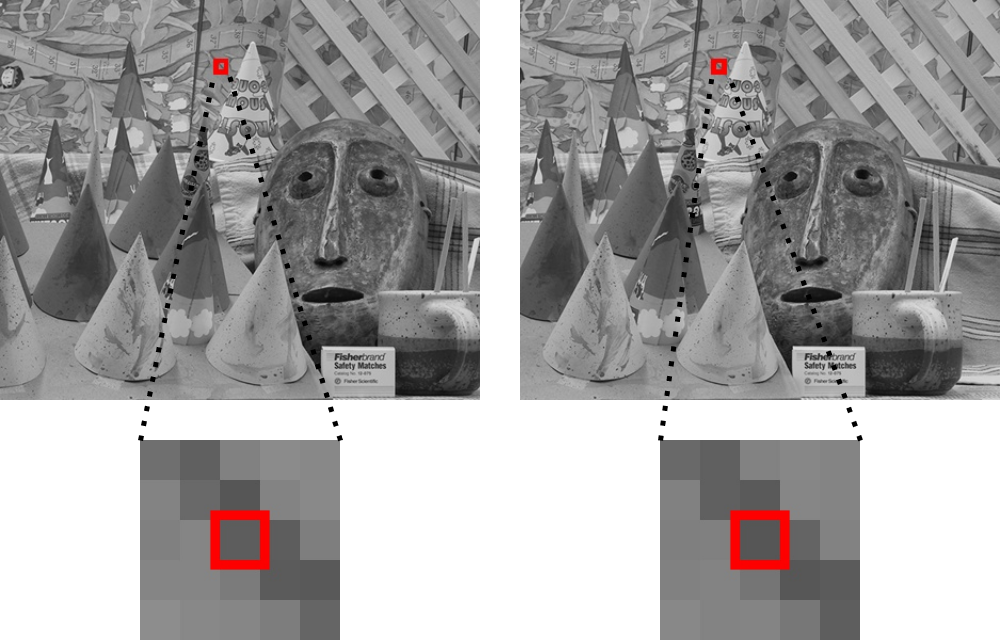
\includegraphics[width=0.8\linewidth]{Images/Cones.png}
  \caption{Homologous pixels in a pair of images}\label{fig:Cones}
\end{figure}

To visualize this uncertainty, we computed upper and lower envelopes for various plausibility levels $\gamma$. These envelopes illustrate the largest (upper bound $\overline{a}$) and smallest (lower bound $\underline{a}$) focal sets where the plausibility, determined by Equation \eqref{eq:bel_pl}, meets or exceeds the given threshold $\gamma$: $\mathrm{Pl}(\overline{a}) \geqslant \gamma$. Consequently, there are two bounds for each level of $\gamma$.
At the plausibility threshold of 0 ($\mathrm{Pl}(\overline{a}) > 0$), the bounds represent the full support of the SAD values. Conversely, at a threshold of 1, the bounds converge to the values of the cost curve obtained in the ``precise'' setting (\ie, without accounting for uncertainty).

\begin{figure}
    \centering
    \begin{subfigure}{0.48\linewidth}
        \centering
        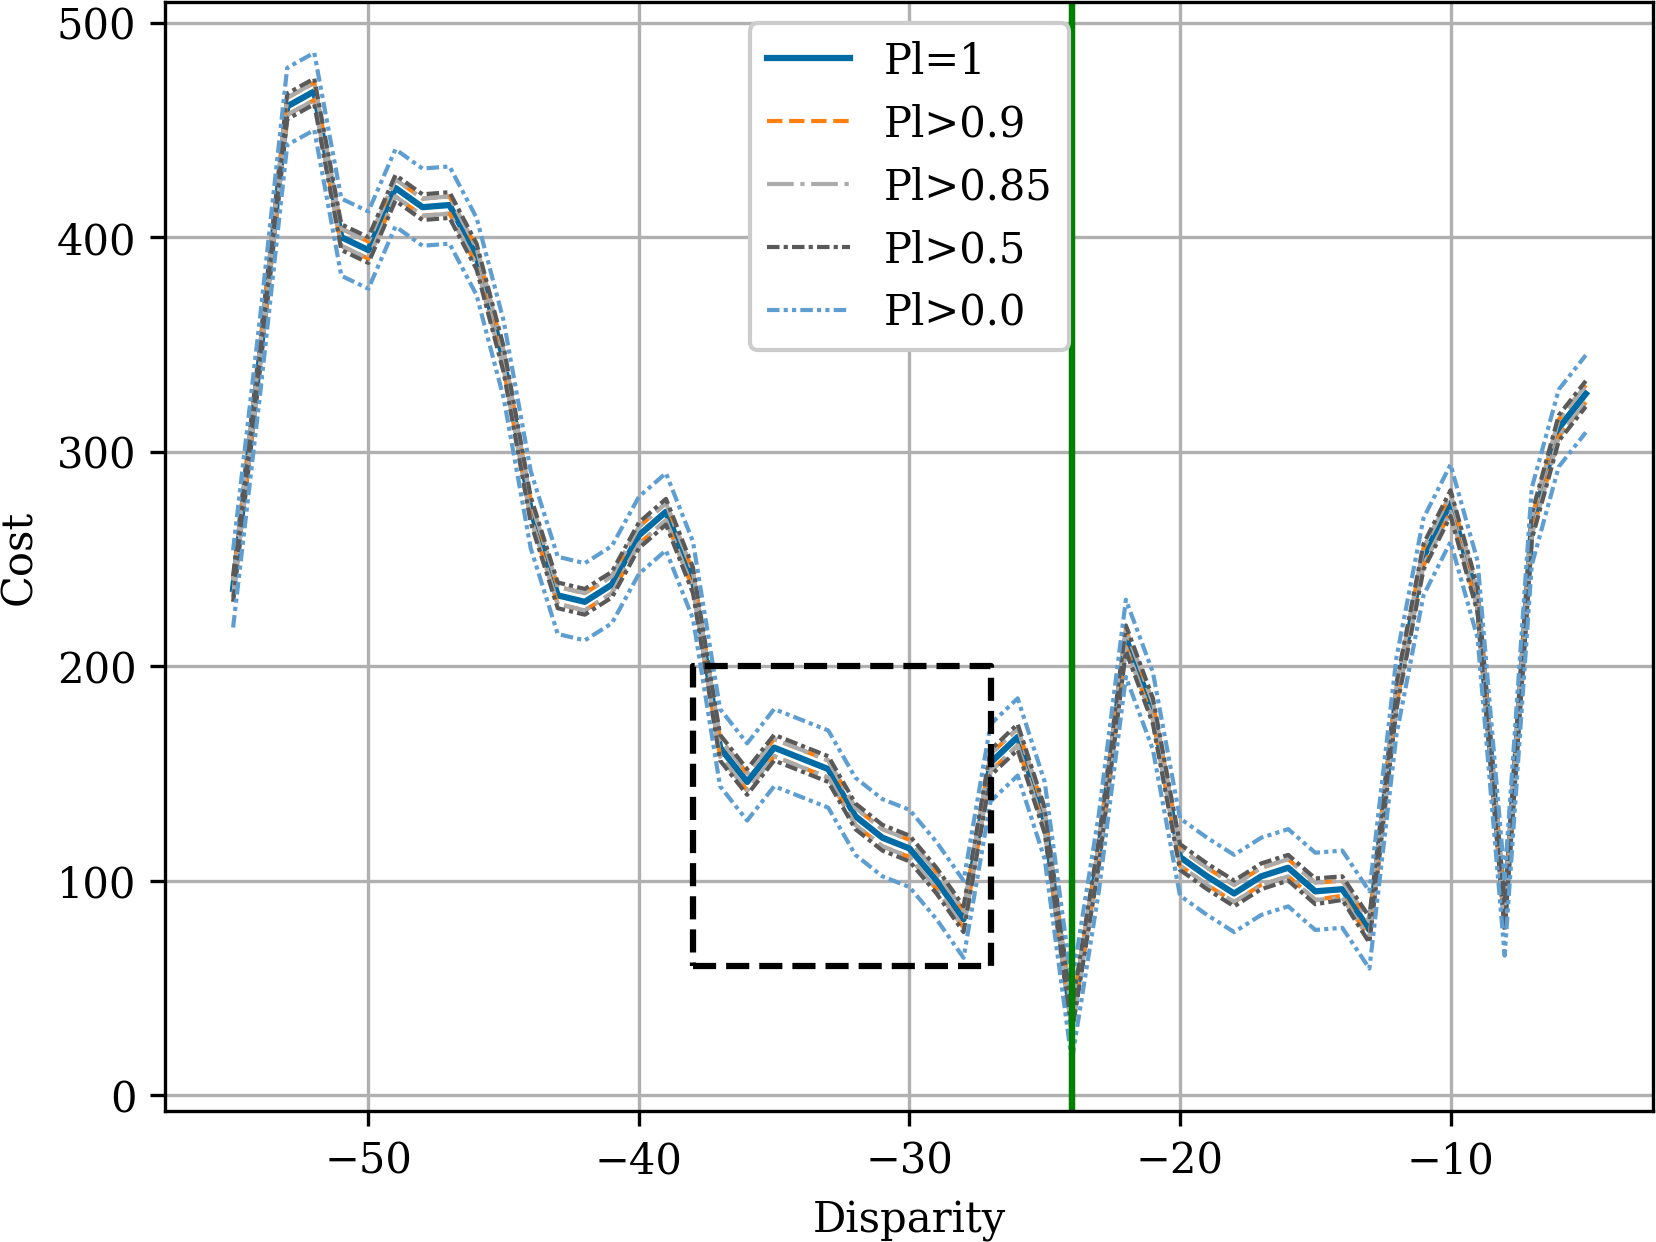
\includegraphics[width=\linewidth]{Images/bel_independence_100_120.png}
        \caption{SAD using the product Copula}
        \label{fig:belief_independence}
    \end{subfigure}\hfill
    \begin{subfigure}{0.48\linewidth}
        \centering
        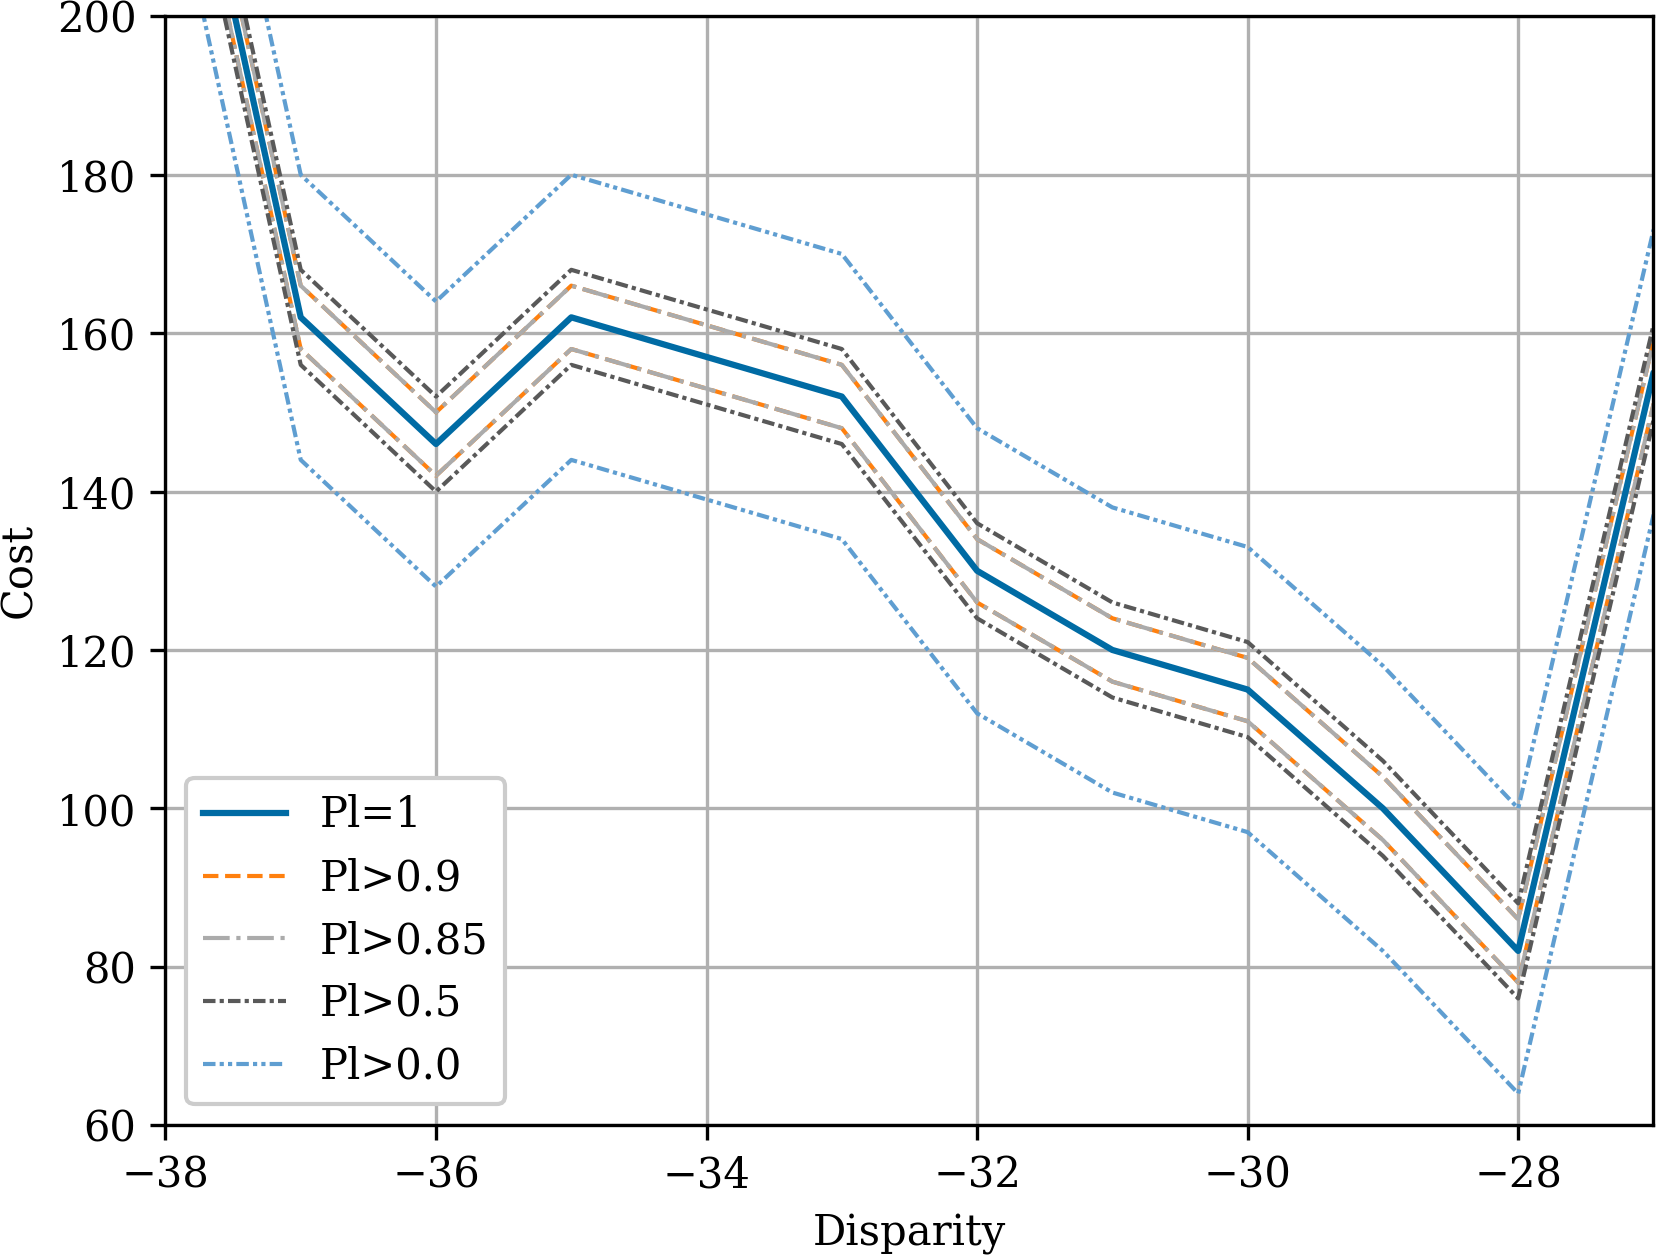
\includegraphics[width=\linewidth]{Images/bel_independence_100_120_zoom.png}
        \caption{Zoom of the rectangle in (a)}
        \label{fig:belief_independence_zoom}
    \end{subfigure}\\
    \begin{subfigure}{0.48\linewidth}
        \centering
        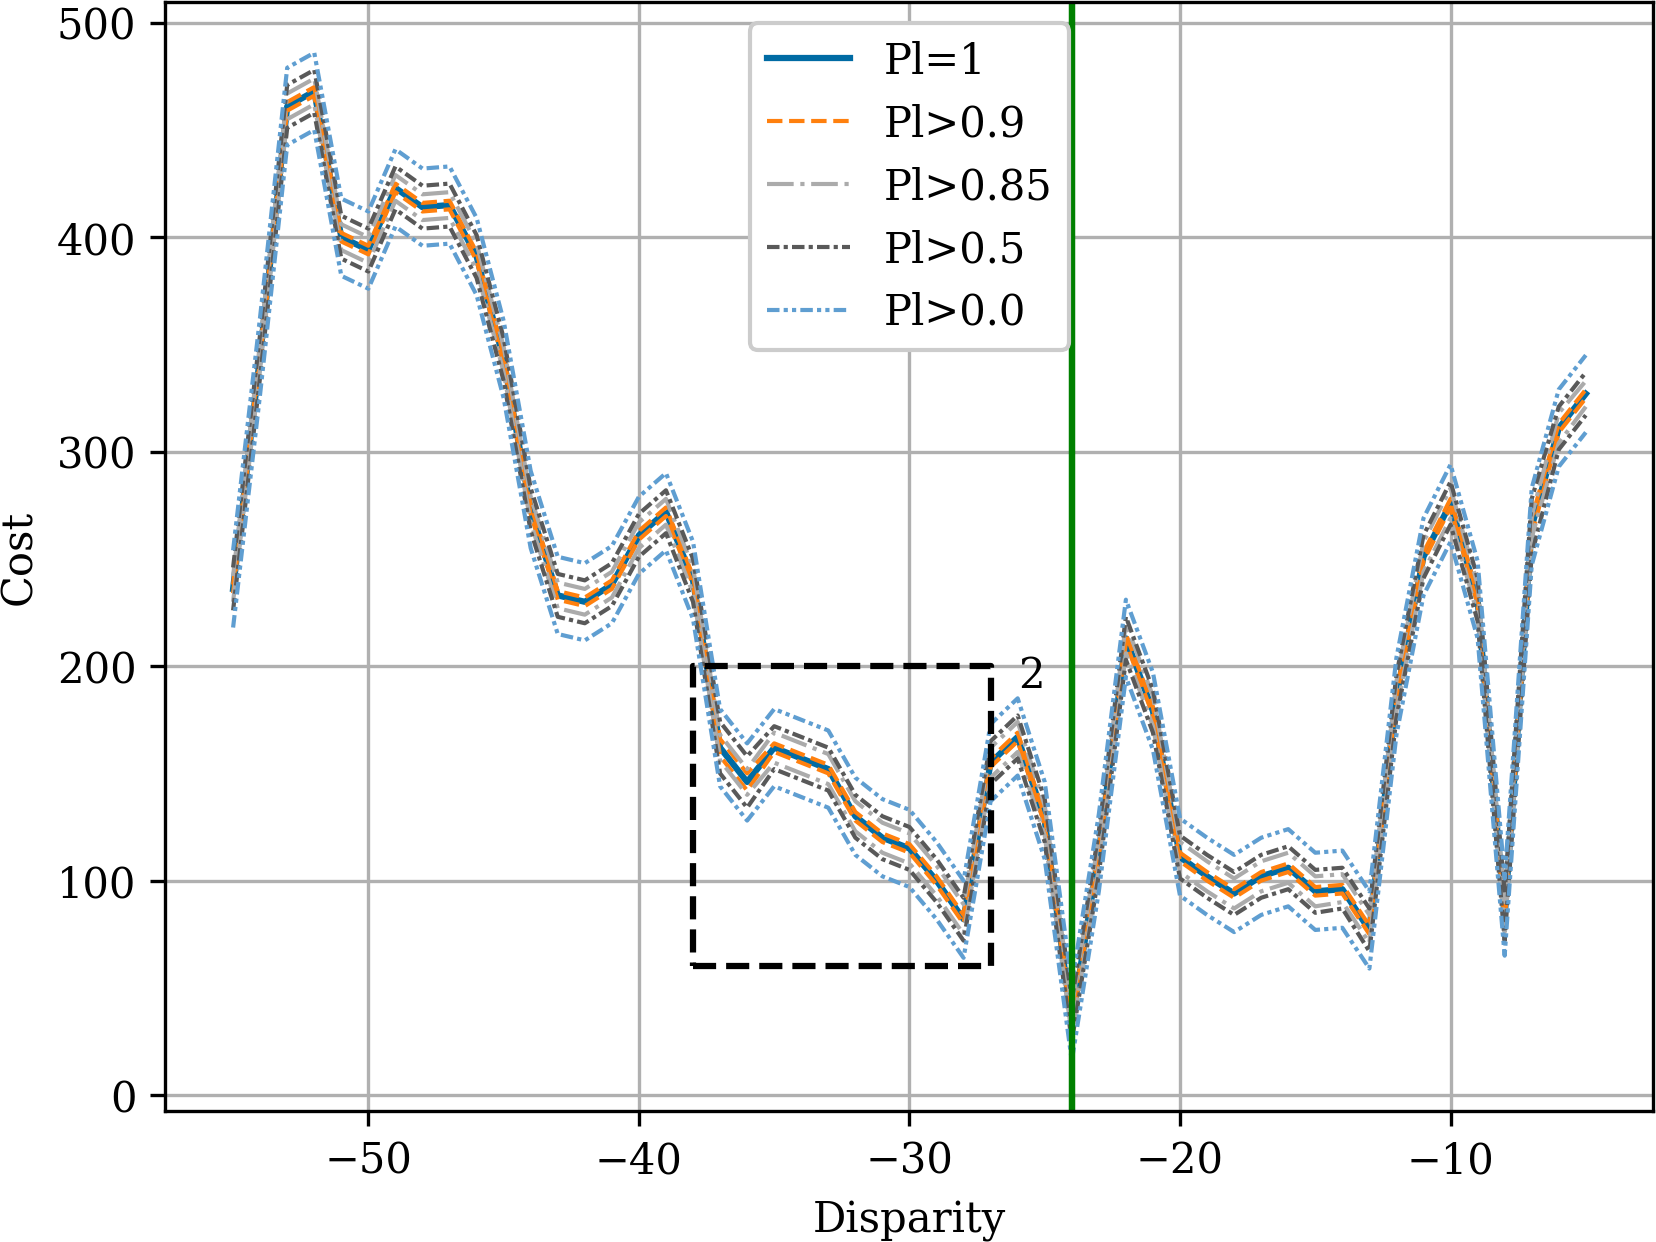
\includegraphics[width=\linewidth]{Images/bel_100_120.png}
        \caption{SAD using the Gaussian Copula}
        \label{fig:belief_gaussian}
    \end{subfigure}\hfill
    \begin{subfigure}{0.48\linewidth}
        \centering
        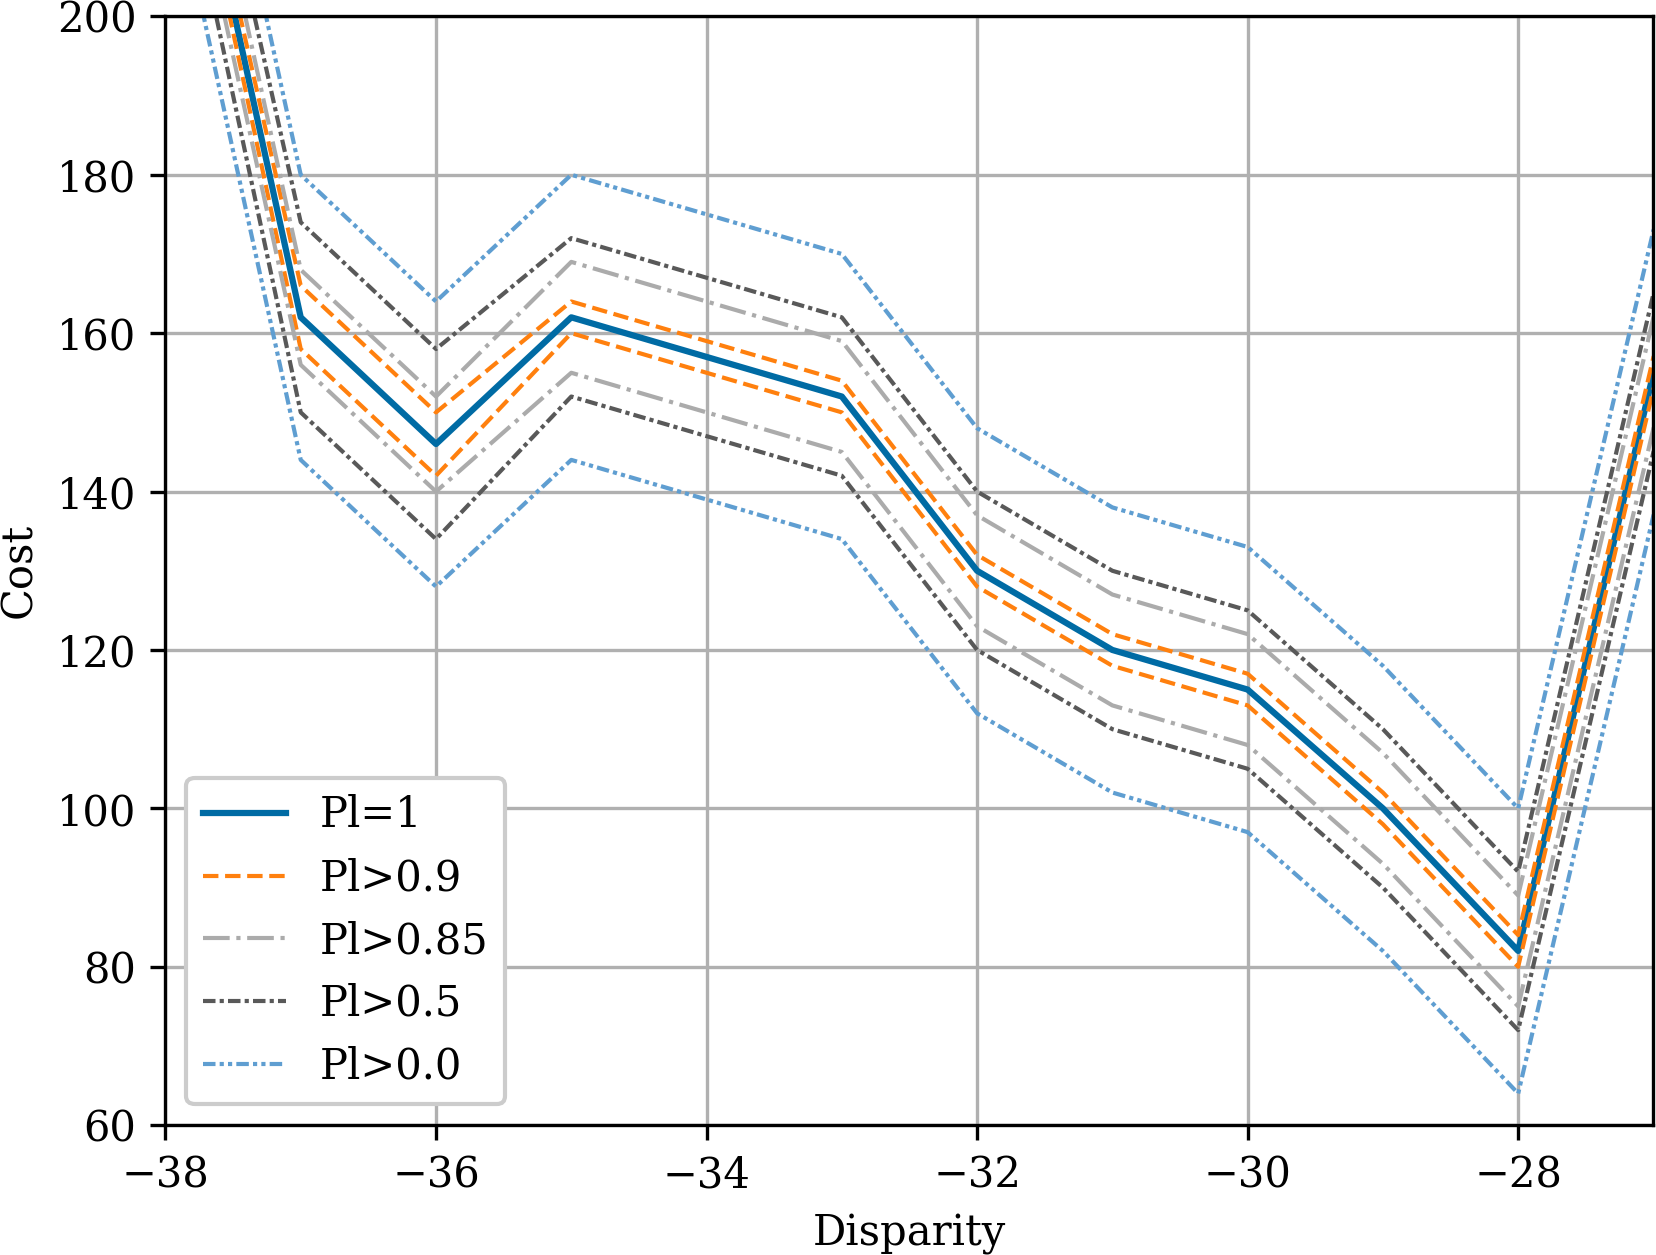
\includegraphics[width=\linewidth]{Images/bel_100_120_zoom.png}
        \caption{Zoom of the rectangle in (c)}
        \label{fig:belief_gaussian_zoom}
    \end{subfigure}
    \caption{Plausibility levels of a cost curve for the product copula $C_\Pi$ and the Gaussian copula $C_R$. The green vertical line represents the true disparity. The figure on the right are a zoom of the black dashed rectangle.}
    \label{fig:belief_curves}
\end{figure}

A visualization of different plausibility levels of the SAD cost curve are presented in figure \ref{fig:belief_curves}, computed with the product copula $C_\Pi$ and a Gaussian copula $C_R$. As both copulas assign non-null masses to the same focal sets, their support ($\mathrm{Pl}>0$) is the same. Taking a copula close to the lower Fréchet-Hoeffding bound (which is not a copula for $n>2$), would lead to a different support, as the image of marginal focal set would be assigned a null mass. Figures \ref{fig:belief_independence_zoom} and \ref{fig:belief_gaussian_zoom} display the fact that the values covered by the plausibility levels vary with the  copula used. The only exception to this concerns the plausibility level $\gamma=1$, corresponding to the SAD curve without noise. The plausibility levels $0.85$ and $0.5$ are more concentrated around plausibility level $1$ in the case of the product copula than in the case of the Gaussian copula. Conversely, plausibility level $0.9$ is closer to plausibility level $1$ in the case of the Gaussian copula. This is due to the fact that the Gaussian copula $C_R$ is more co-monotone than the product copula, given the correlation matrix $R$ described in \eqref{eq:correlation}.

\section{Estimating Propagated Credal Sets Using Monte Carlo Sampling}
In order to evaluate the validity of the propagated belief functions, we try to estimate $\M_{robust}$ using Monte Carlo samplings. We first generate probability distributions belonging in the marginal credal sets. This sampling is not random as we generate probability distributions in such a way that the probability range on events imposed by the marginal possibility distributions is uniformly covered. We also make sure that lower and upper bounds on events are all reached at least once, in order to include ``extreme'' distributions in our simulations. Once every marginal probability distribution of every pixel used to compute a cost curve has been sampled, we can generate random samples from their joint distribution. We thus generate samples from the copula and marginals as detailed in section \ref{sec:sampling_copula}. This yields noised version of patches from the left images, where the noised samples dependency is modeled by the provided copula. Finally, we compute the cost curves using those random images, giving us Monte Carlo samples of the SAD cost curves for a given copula.

Note that we could simulate a single version of the noised pair of images, but that would require to sample from a copula of very large dimension (the number of pixels in both images). This is not realistically feasible, even thought it would ensure that the same version of noised pixels are used in all cost curves (or in other words, for a single draw, the noised intensities will not change depending on the cost curve computed). We instead generate noise samples for each row separately: noised values of pixels will not change during the evaluation of a cost curve for different disparities, or between the cost curves of pixels of the same row. However, their values might change between cost curves of pixels belonging to different rows. For instance, let's consider a pixel $p=(row,~col)\in I_L$ for which we computed a noised intensity $i_p$. Then we will use the same noised value $i_p$ of intensity when computing the SAD of every pixel $q=(row,~col')\in I_L$. But when computing the SAD of every pixel $q=(row-1,~col')\in I_L$, we will use a different Monte Carlo draw for the value $i_p$, which will stay the same for every pixel of row $row-1$. Because we draw a high number of Monte Carlo draws ($10,000$) for each row, the effect of this of proceeding should not be noticeable. 

Monte Carlo draws using the Gaussian copula and marginals credal sets of \ref{eq:pixel_possibility} are plotted in figures \ref{fig:montecarlo_gauss_100_120} and \ref{fig:montecarlo_gauss_200_150}. Different plausibility levels, similar to those of figures \ref{fig:belief_curves}, also appear for comparison. The support envelopes from plausibility levels $\mathrm{Pl}>0$ correctly contain all Monte Carlo samplings for all considered copulas. We can observe in Figure \ref{fig:montecarlo_gauss_200_150_zoom2} that plausibility levels sometimes fail to correctly grasp the fluctuations of the dispersion of the samples, even though they seem to correctly contain Monte Carlo samples. For instance, Monte Carlo draws are first dense around disparity $-37$, then seem to spread around $-35$, and finally regather around disparity $-32$. The plausibility envelopes are more regular in this disparity range. This illustrates the fact the ``true'' point-wise credal $\M_{robust}$ set described in section \ref{sec:robust_method} and approximated with Monte Carlo samples is different from that the joint credal set $\M_{mass}$ from section \ref{sec:joint_mass}. Although some differences persist between those sets, Figure \ref{fig:montecarlo_gauss_100_120_zoom2} or \ref{fig:montecarlo_gauss_200_150_zoom2} suggest that Monte Carlo simulations can correctly estimate the point-wise credal set $\M_{robust}$ by joining belief functions using a copula as in equation \eqref{eq:joint_mass}. This is furthermore justified by the  quantitative analysis presented in Table \ref{tab:Coverage}, where the proportion of Monte Carlo samplings contained inside the plausibility envelopes, is computed for different plausibility levels $\gamma$. We will call this proportion ``coverage''. The coverage for figures \ref{fig:montecarlo_gauss_100_120} and \ref{fig:montecarlo_gauss_200_150} are presented in the first and second rows of Table \ref{tab:Coverage} respectively. The global coverage over the whole left image is presented in the last row of the table. The coverage is always $100\%$ for $\gamma=0$, which indicates that every sample is contained inside the support envelopes. \todoroman{Je pense que ce que je dis ensuite est faux. Le coverage ne donne pas d'indication sur les plausibility estimées, car celles ci ne retranscrivent pas une fréquence mais seulement un niveau de croyance. Comment donner une interprétation correcte de la densité?} As envelopes are defined as lower and upper bounds of the focal sets with a plausibility superior to $\gamma$, the coverage should be superior to $1-\gamma$, which is indeed the case.

\begin{figure}
    \centering
    \begin{subfigure}{1\linewidth}
        \centering
        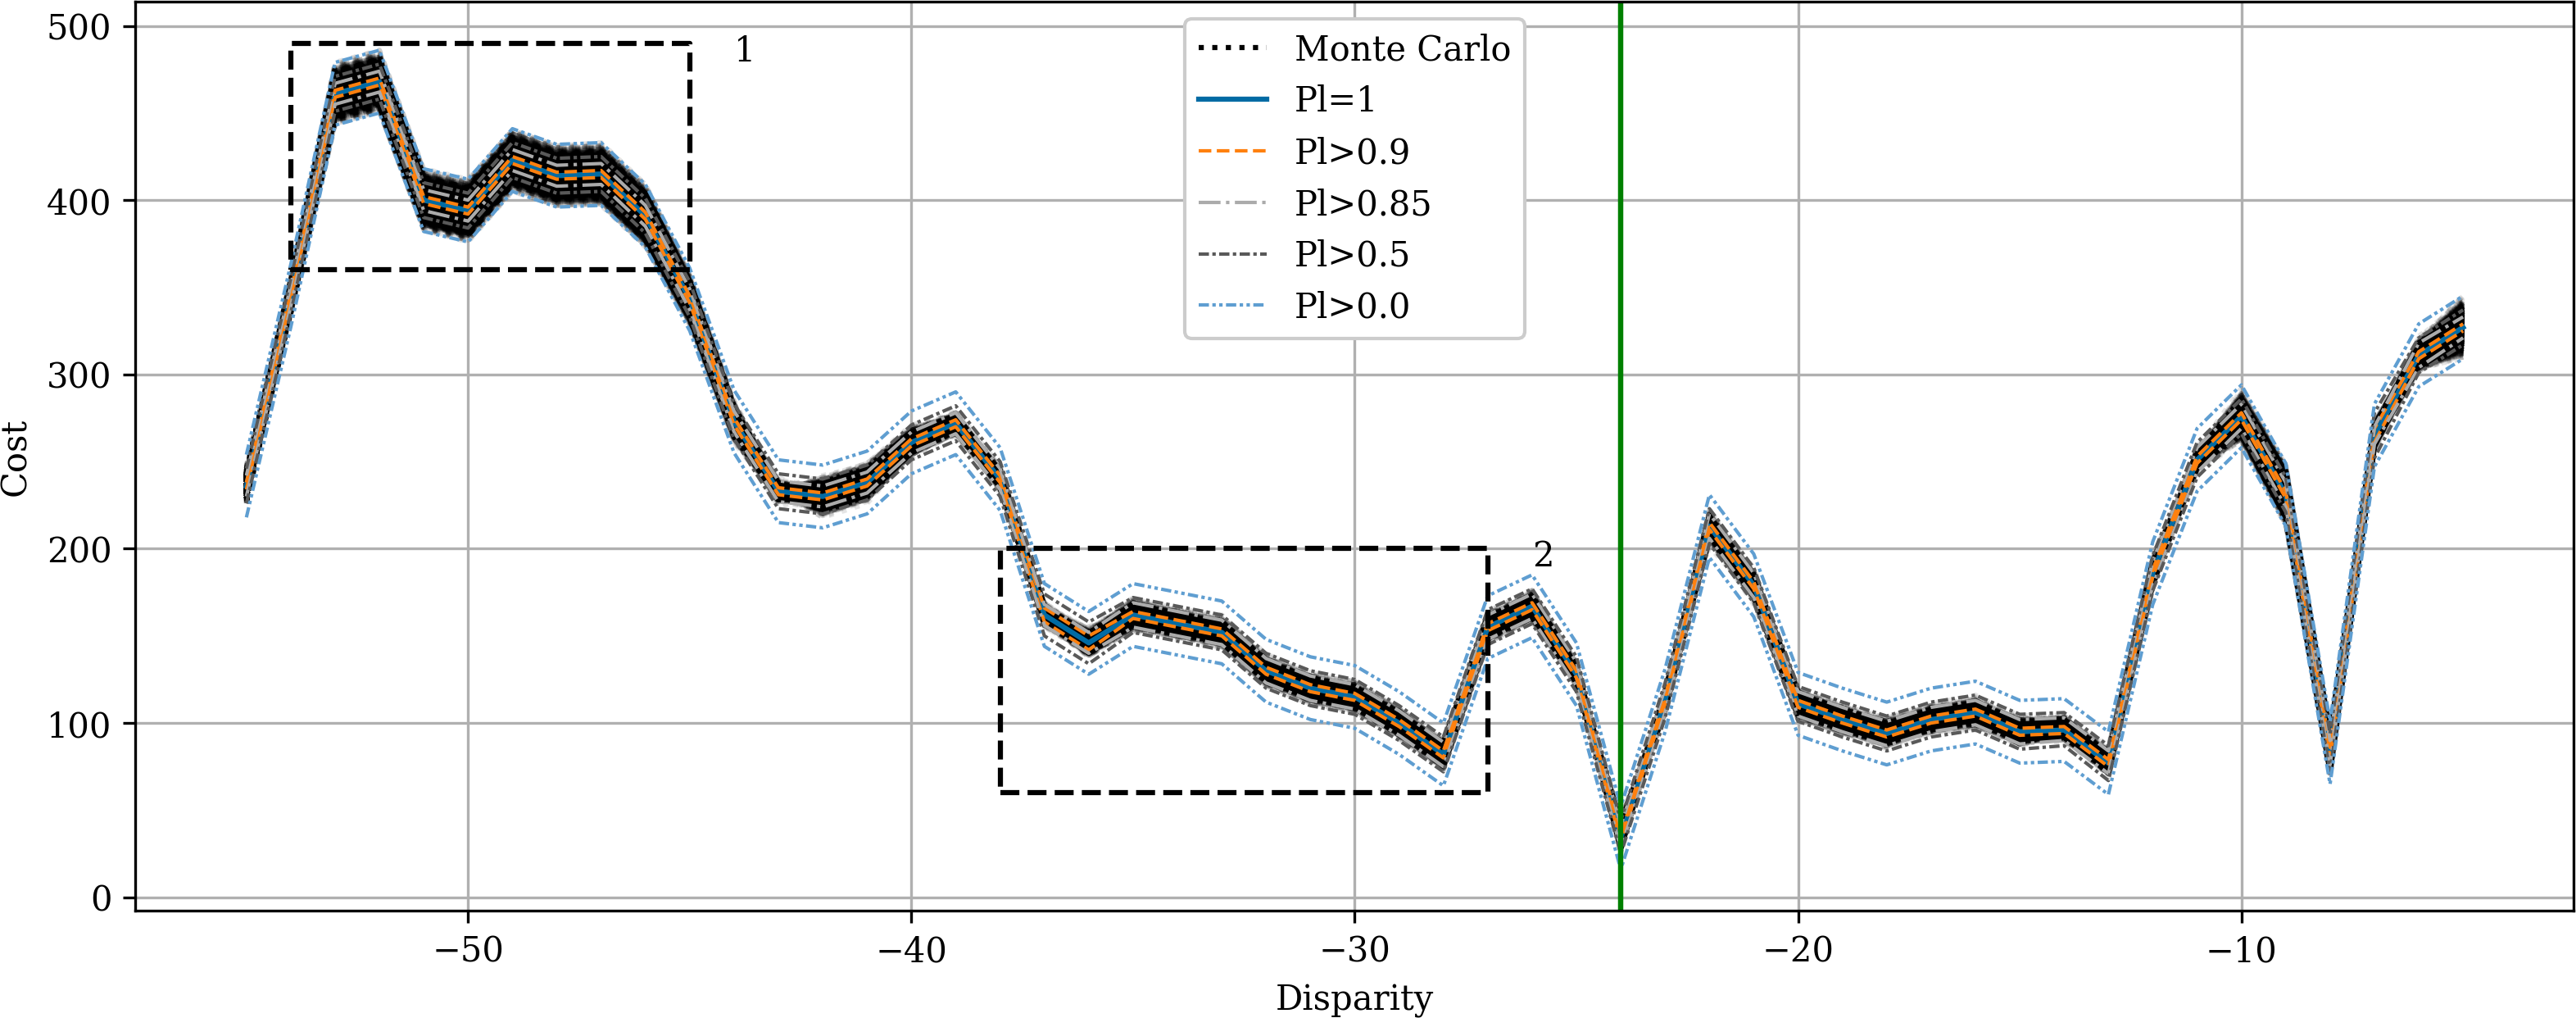
\includegraphics[width=\linewidth]{Images/cost_curve_100_120.png}
        \caption{Plausibility levels and Monte Carlo sampling using a Gaussian copula}
        \label{fig:montecarlo_gauss_100_120_large}
    \end{subfigure}\\
    \begin{subfigure}{0.45\linewidth}
        \centering
        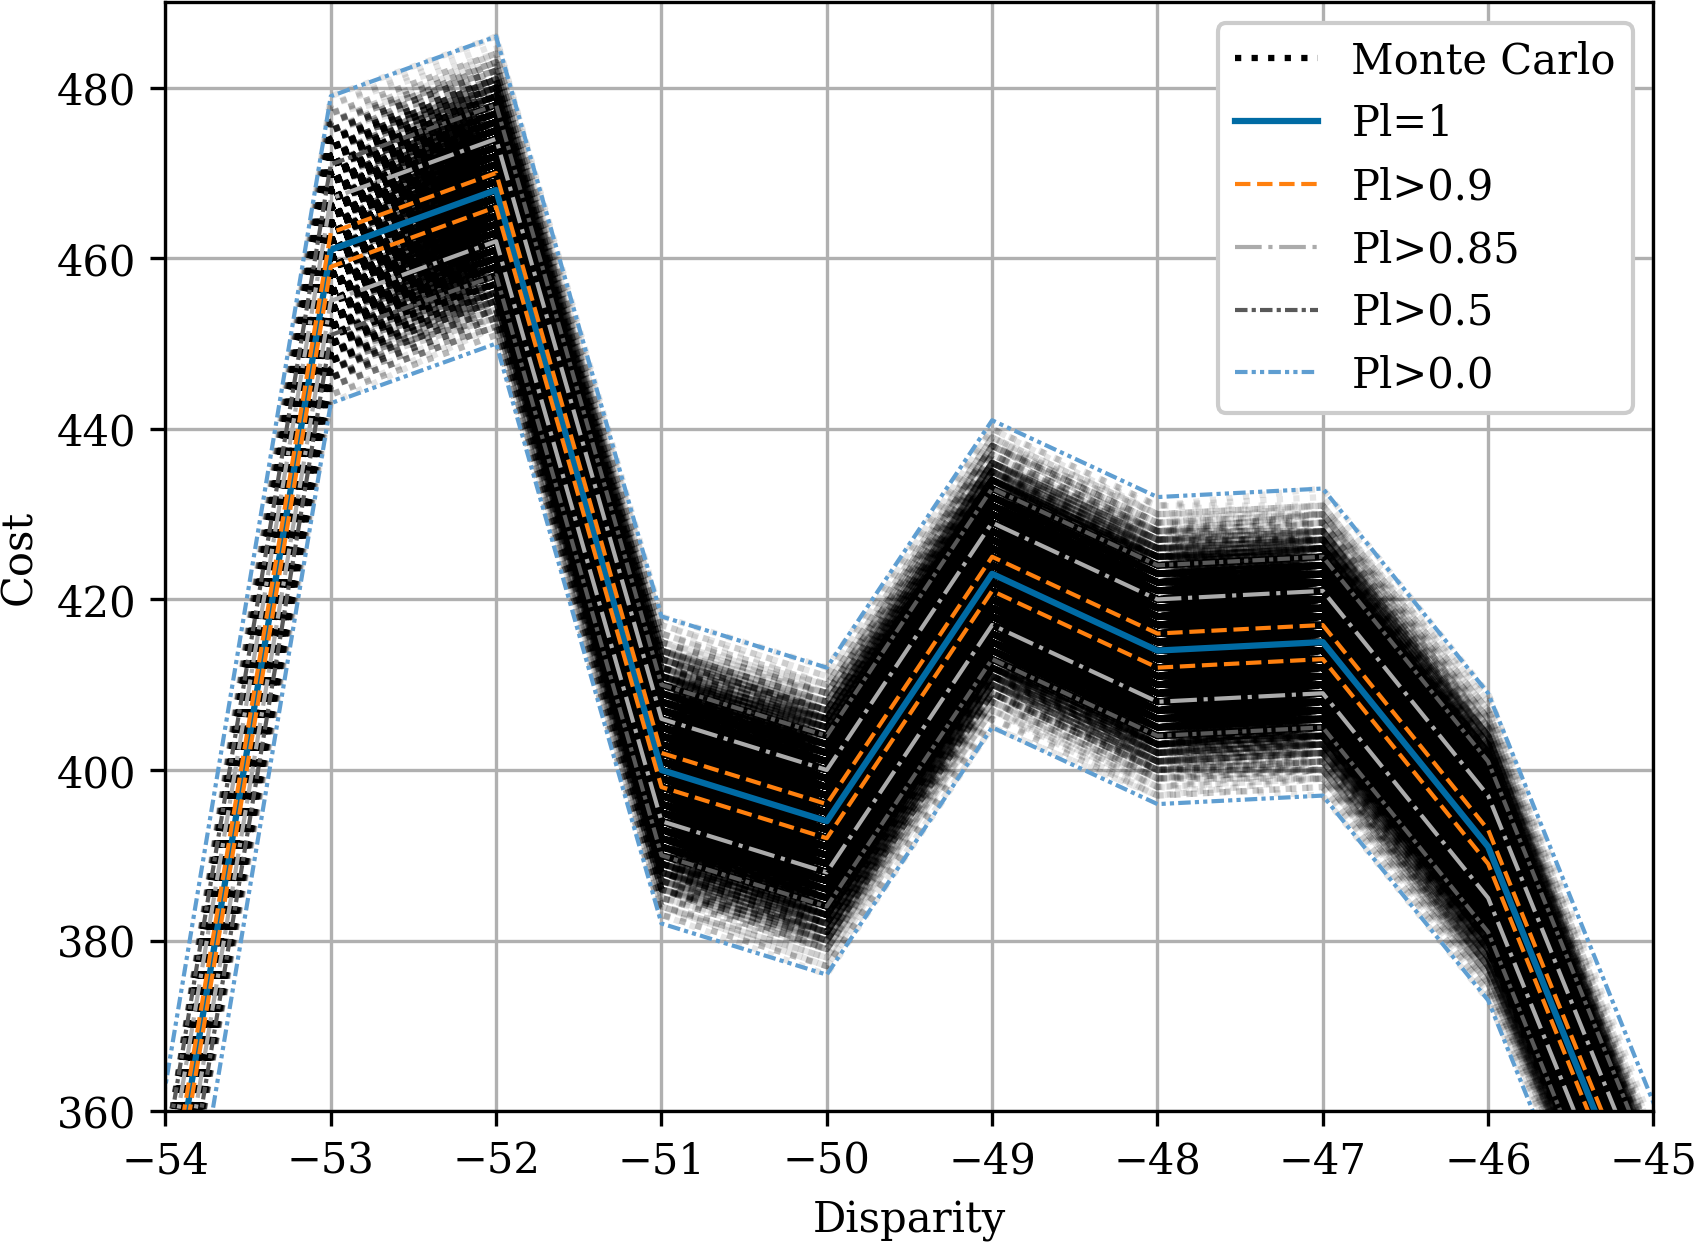
\includegraphics[width=\linewidth]{Images/cost_curve_100_120_zoom1.png}
        \caption{Zoom over the first rectangle}
        \label{fig:montecarlo_gauss_100_120_zoom1}
    \end{subfigure}\hfill
    \begin{subfigure}{0.45\linewidth}
        \centering
        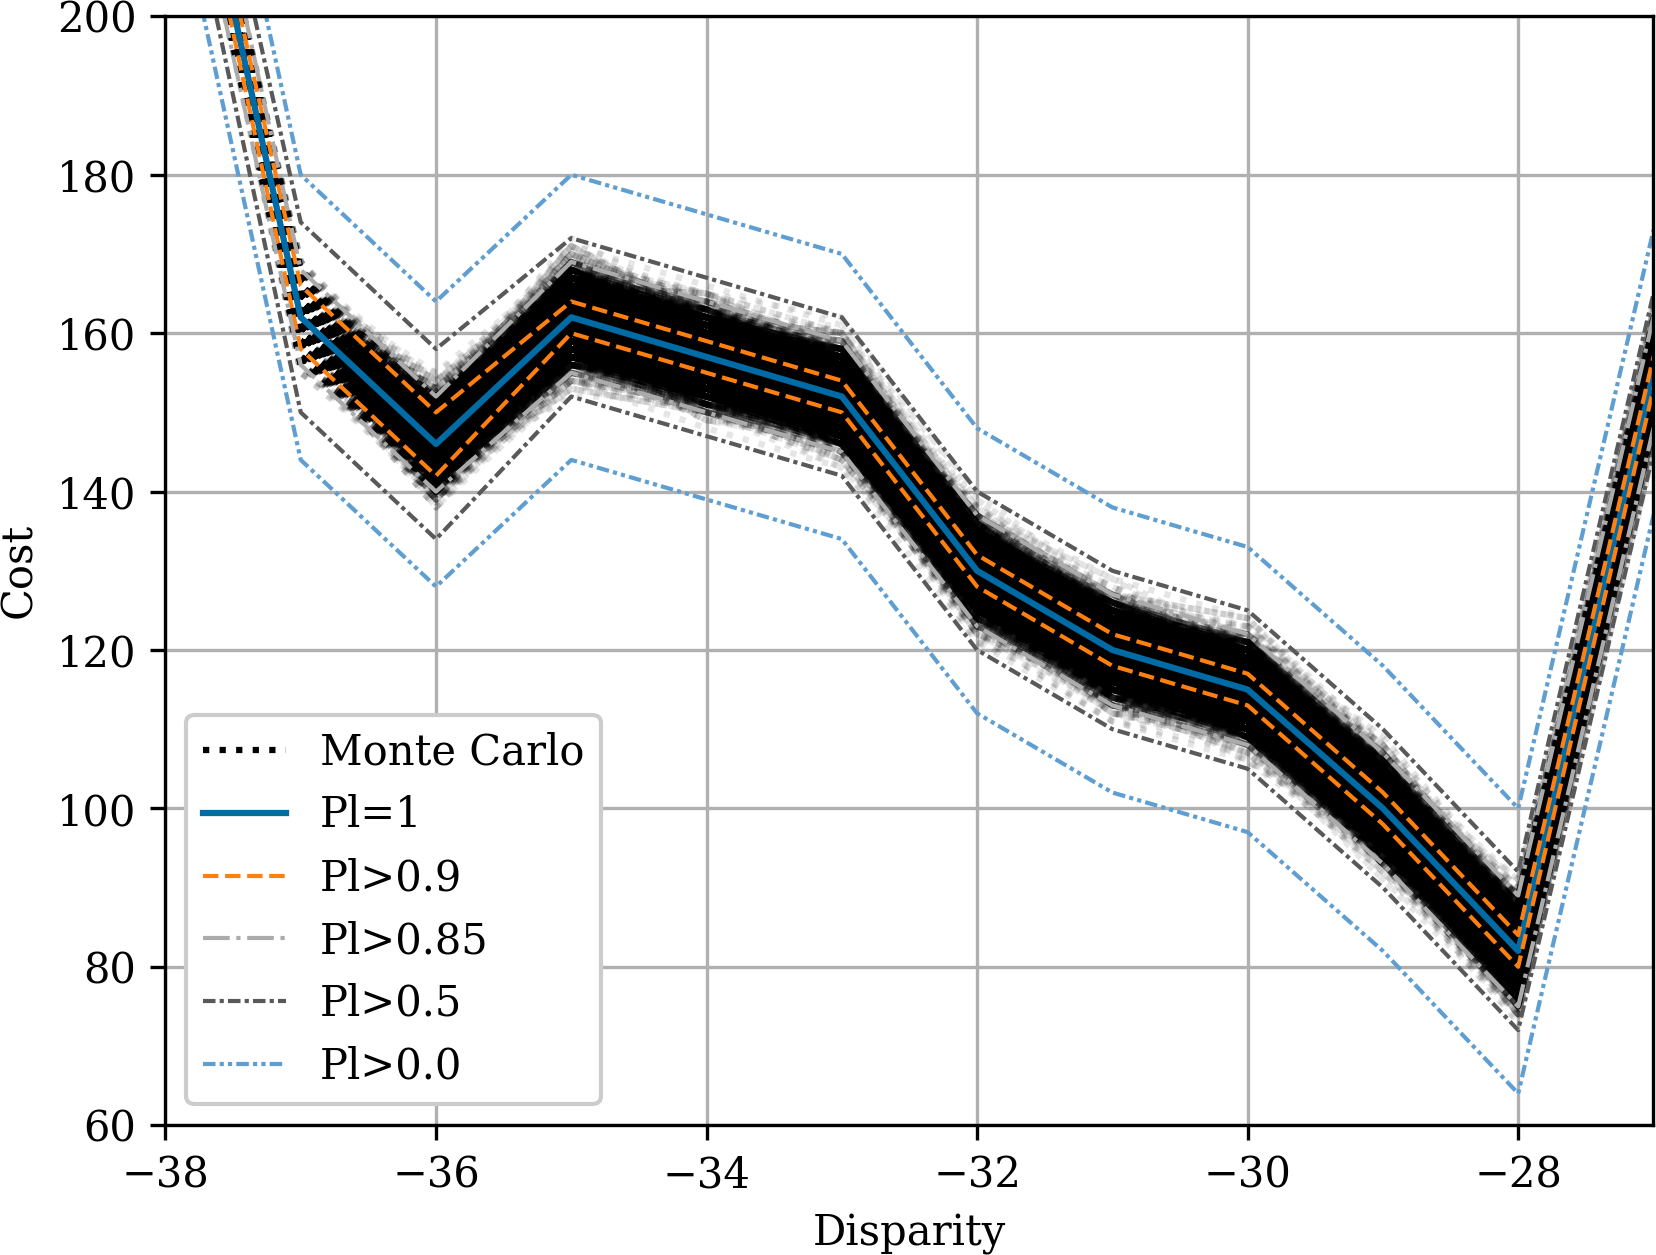
\includegraphics[width=\linewidth]{Images/cost_curve_100_120_zoom2.png}
        \caption{Zoom over the second rectangle}
        \label{fig:montecarlo_gauss_100_120_zoom2}
    \end{subfigure}
    \caption{Plausibility levels and Monte Carlo sampling for a pixel of the left image}
    \label{fig:montecarlo_gauss_100_120}
\end{figure}

\begin{figure}
    \centering
    \begin{subfigure}{\linewidth}
        \centering
        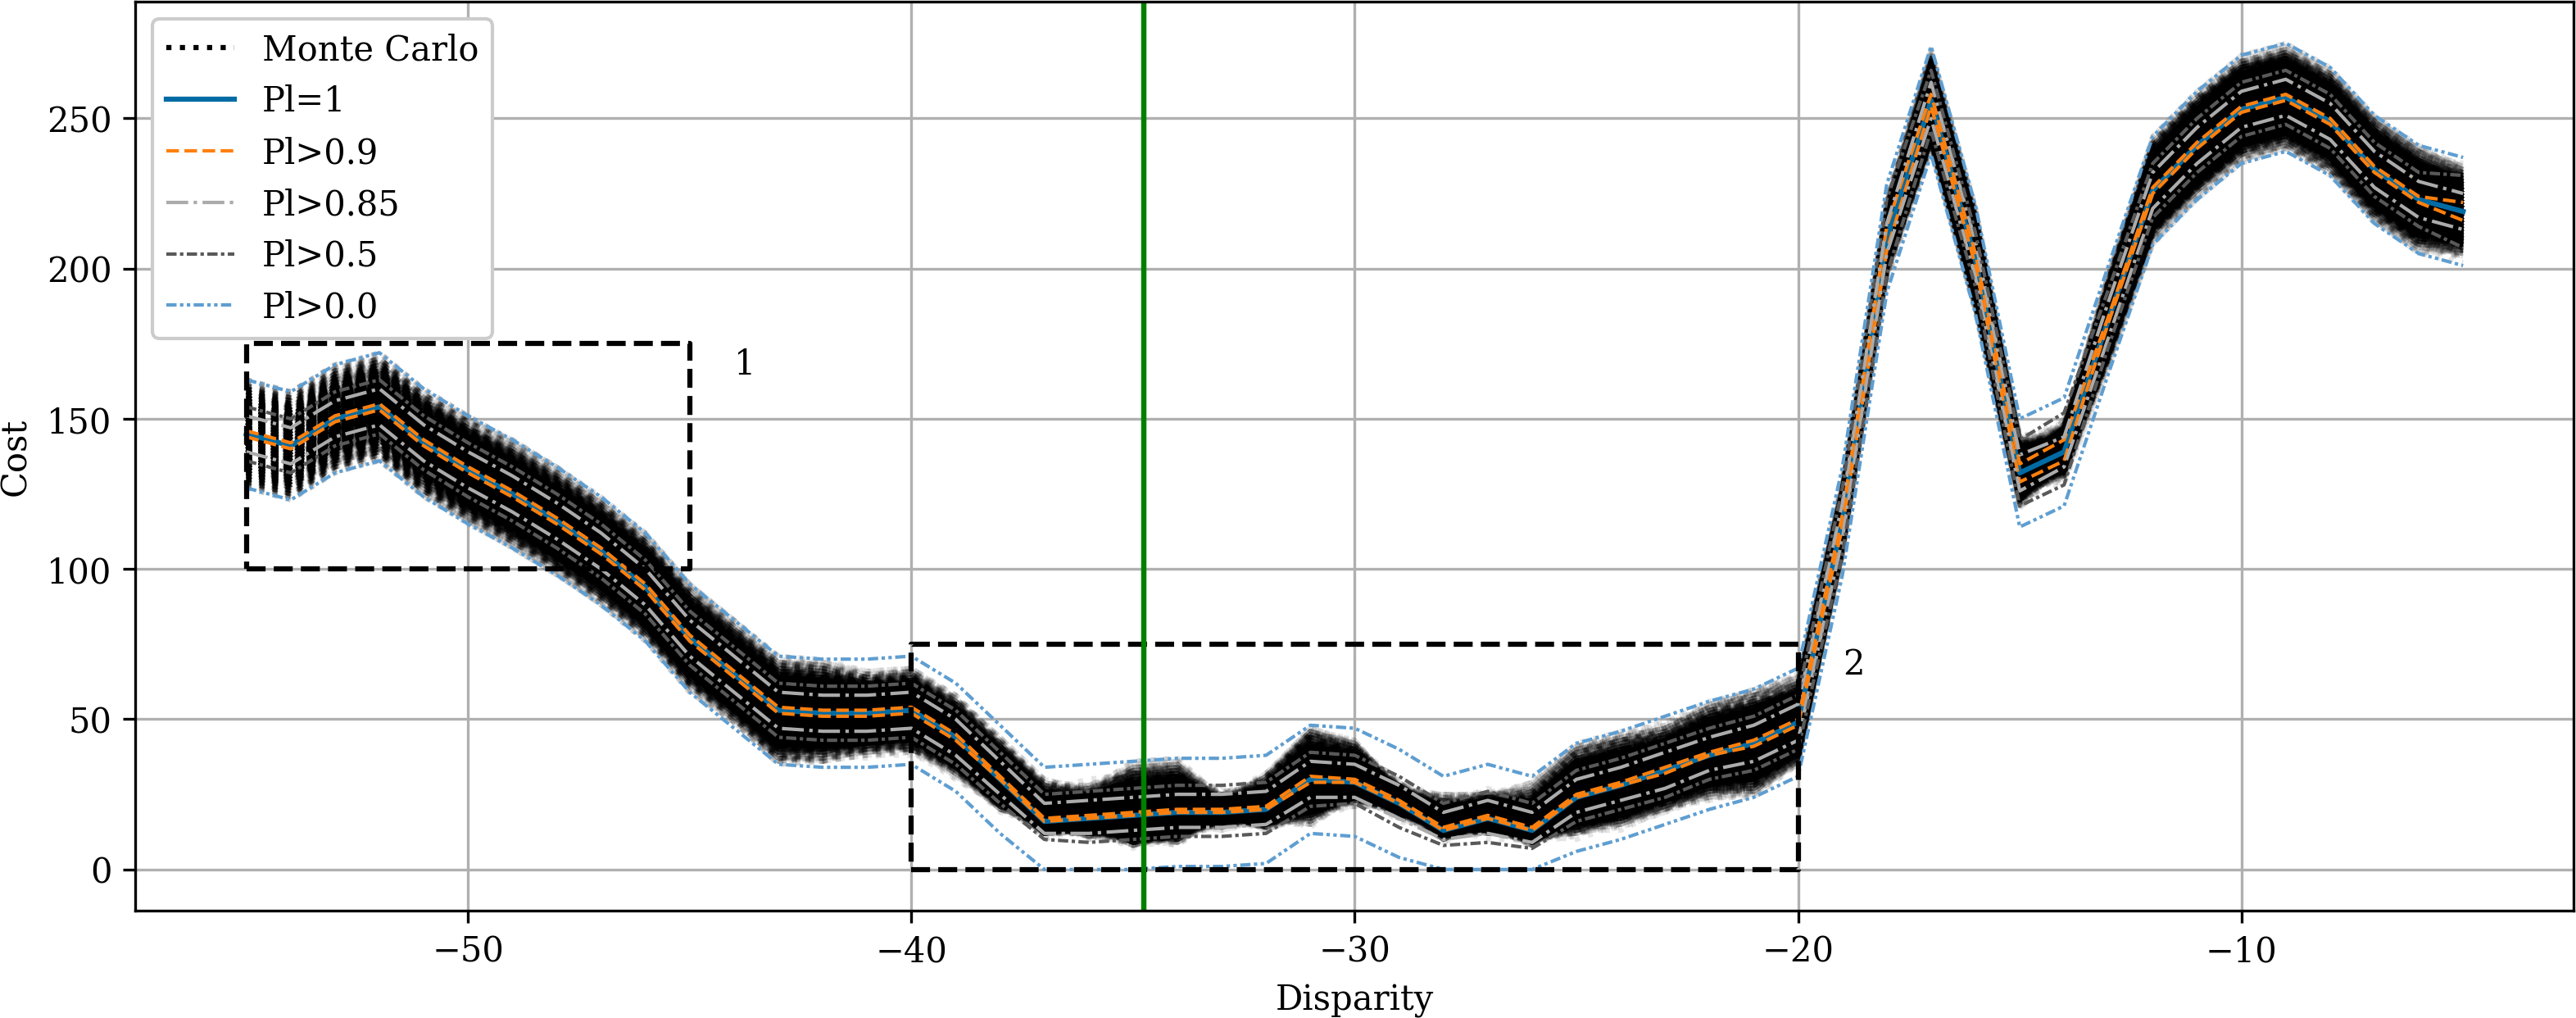
\includegraphics[width=\linewidth]{Images/cost_curve_200_150.png}
        \caption{Plausibility levels and Monte Carlo sampling using a Gaussian copula}
        \label{fig:montecarlo_gauss_200_150_large}
    \end{subfigure}\\
    \begin{subfigure}{0.45\linewidth}
        \centering
        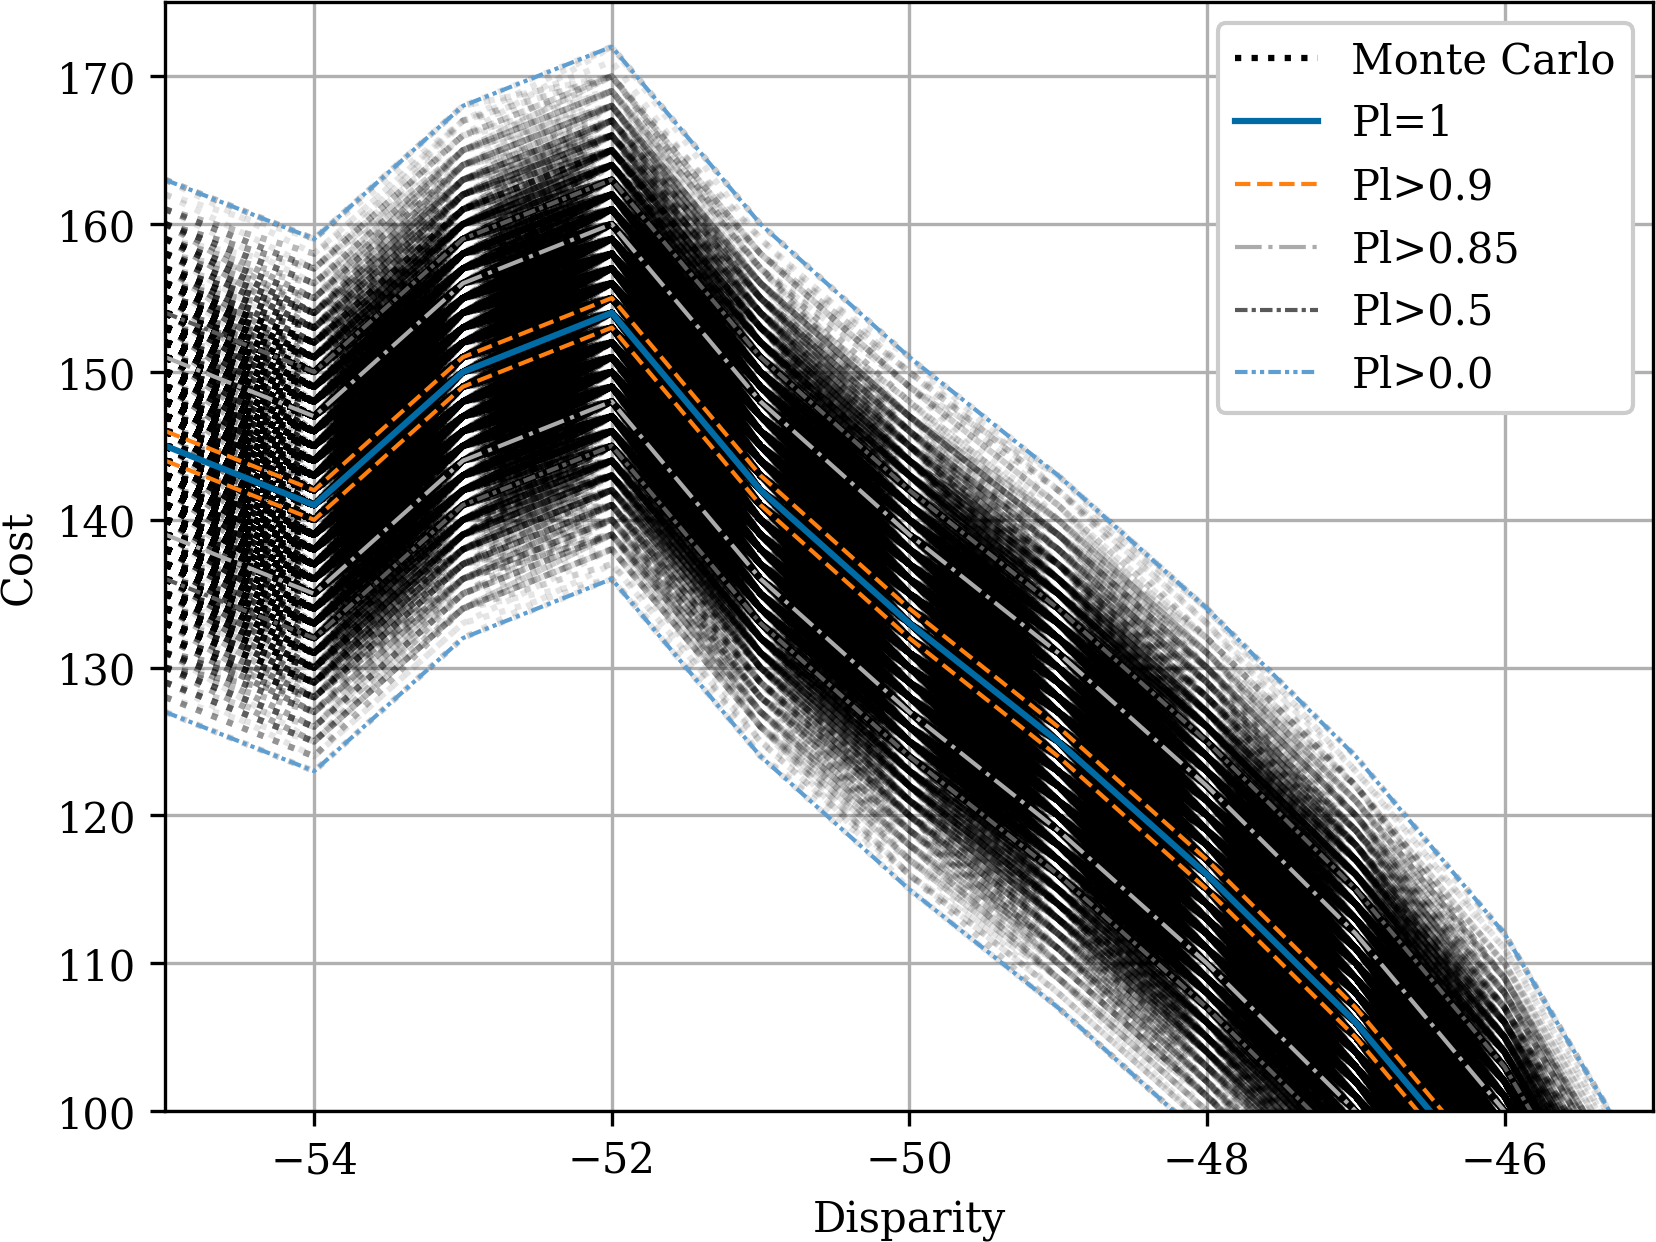
\includegraphics[width=\linewidth]{Images/cost_curve_200_150_zoom1.png}
        \caption{Zoom over the first rectangle}
        \label{fig:montecarlo_gauss_200_150_zoom1}
    \end{subfigure}
    \hfill
    \begin{subfigure}{0.45\linewidth}
        \centering
        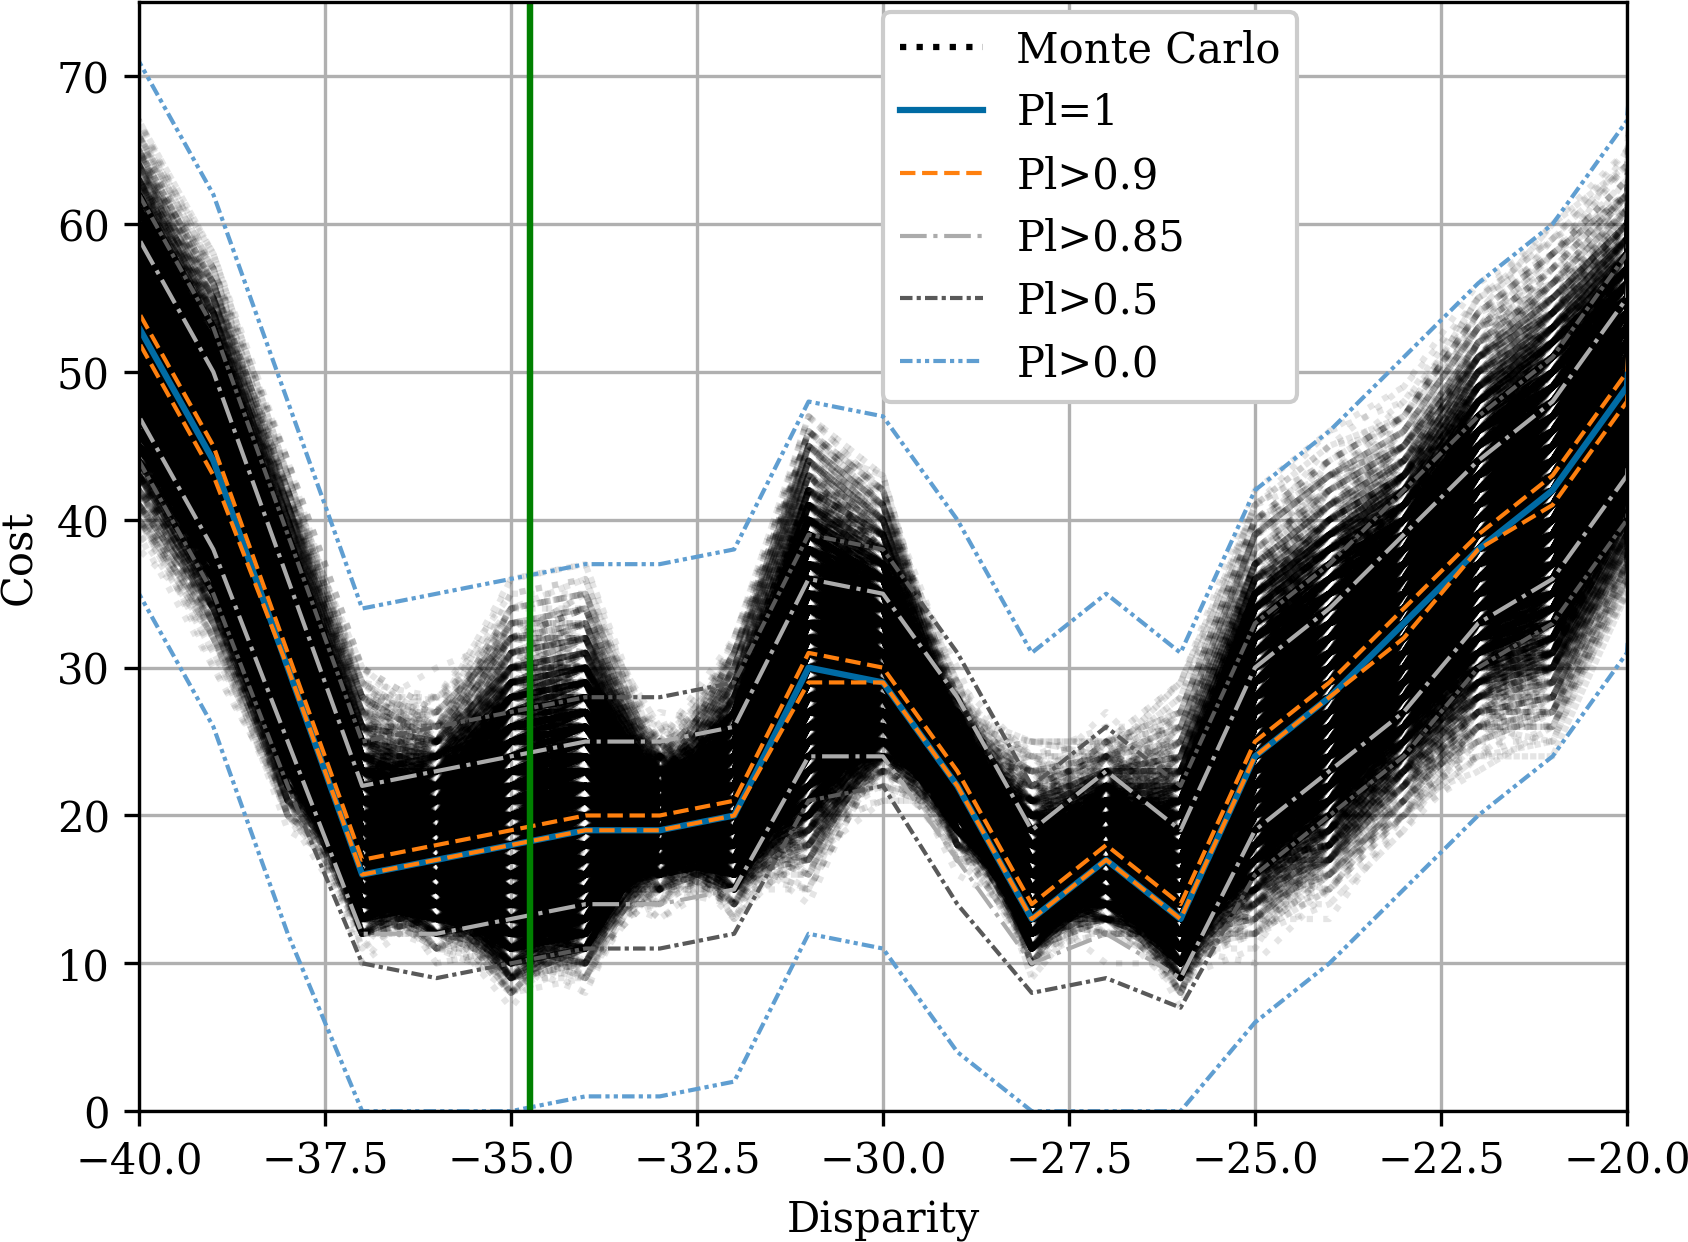
\includegraphics[width=\linewidth]{Images/cost_curve_200_150_zoom2.png}
        \caption{Zoom over the second rectangle}
        \label{fig:montecarlo_gauss_200_150_zoom2}
    \end{subfigure}
    \caption{Plausibility levels and Monte Carlo sampling for a pixel of the left image}
    \label{fig:montecarlo_gauss_200_150}
\end{figure}

\begin{table}[ht]
\centering
\begin{tabular}{|c|c|c|c|c|}
\hline
\rowcolor[HTML]{C0C0C0}
$p=(row,col)$ & $\gamma=0.9$  & $\gamma=0.85$ & $\gamma=0.5$  & $\gamma=0$   \\ \hline
\cellcolor[HTML]{C0C0C0}$(100,~120)$     & $64,5\%$ & $94,5\%$ & $99,0\%$ & $100\%$ \\ \hline
\cellcolor[HTML]{C0C0C0}$(200,~150)$     & $30,0\%$ & $82,6\%$ & $95,2\%$ & $100\%$ \\ \hline
\cellcolor[HTML]{C0C0C0}Global        & $41,1\%$ & $87,6\%$ & $96,8\%$ & $100\%$ \\ \hline
\end{tabular}
\caption{Average coverage for various plausibility levels $\gamma$ and for different pixels $p$ of the left image.}\label{tab:Coverage}
\end{table}

\begin{figure}[ht]
    \centering
    \begin{subfigure}{0.48\linewidth}
        \centering
        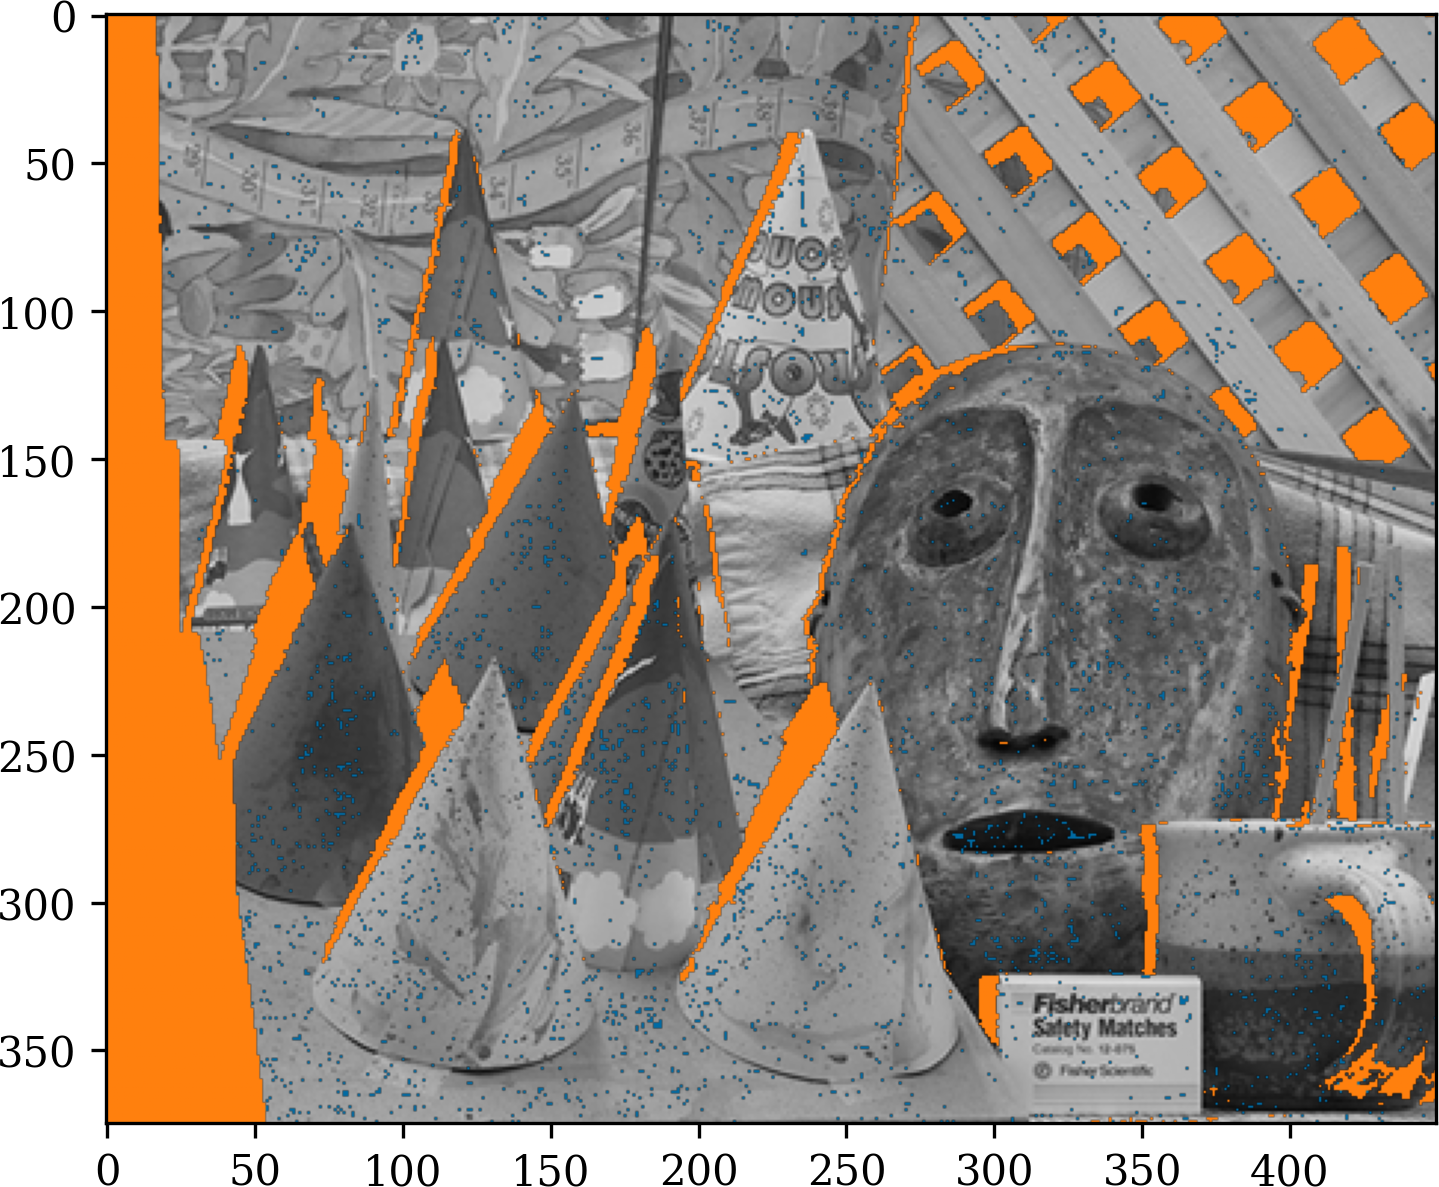
\includegraphics[width=\linewidth]{Images/Improvements_Pl=0.9.png}
        \caption{$\gamma=0.9,~\Delta s_\gamma=4.05\%$}
        \label{fig:improvements_a}
    \end{subfigure}
    \begin{subfigure}{0.48\linewidth}
        \centering
        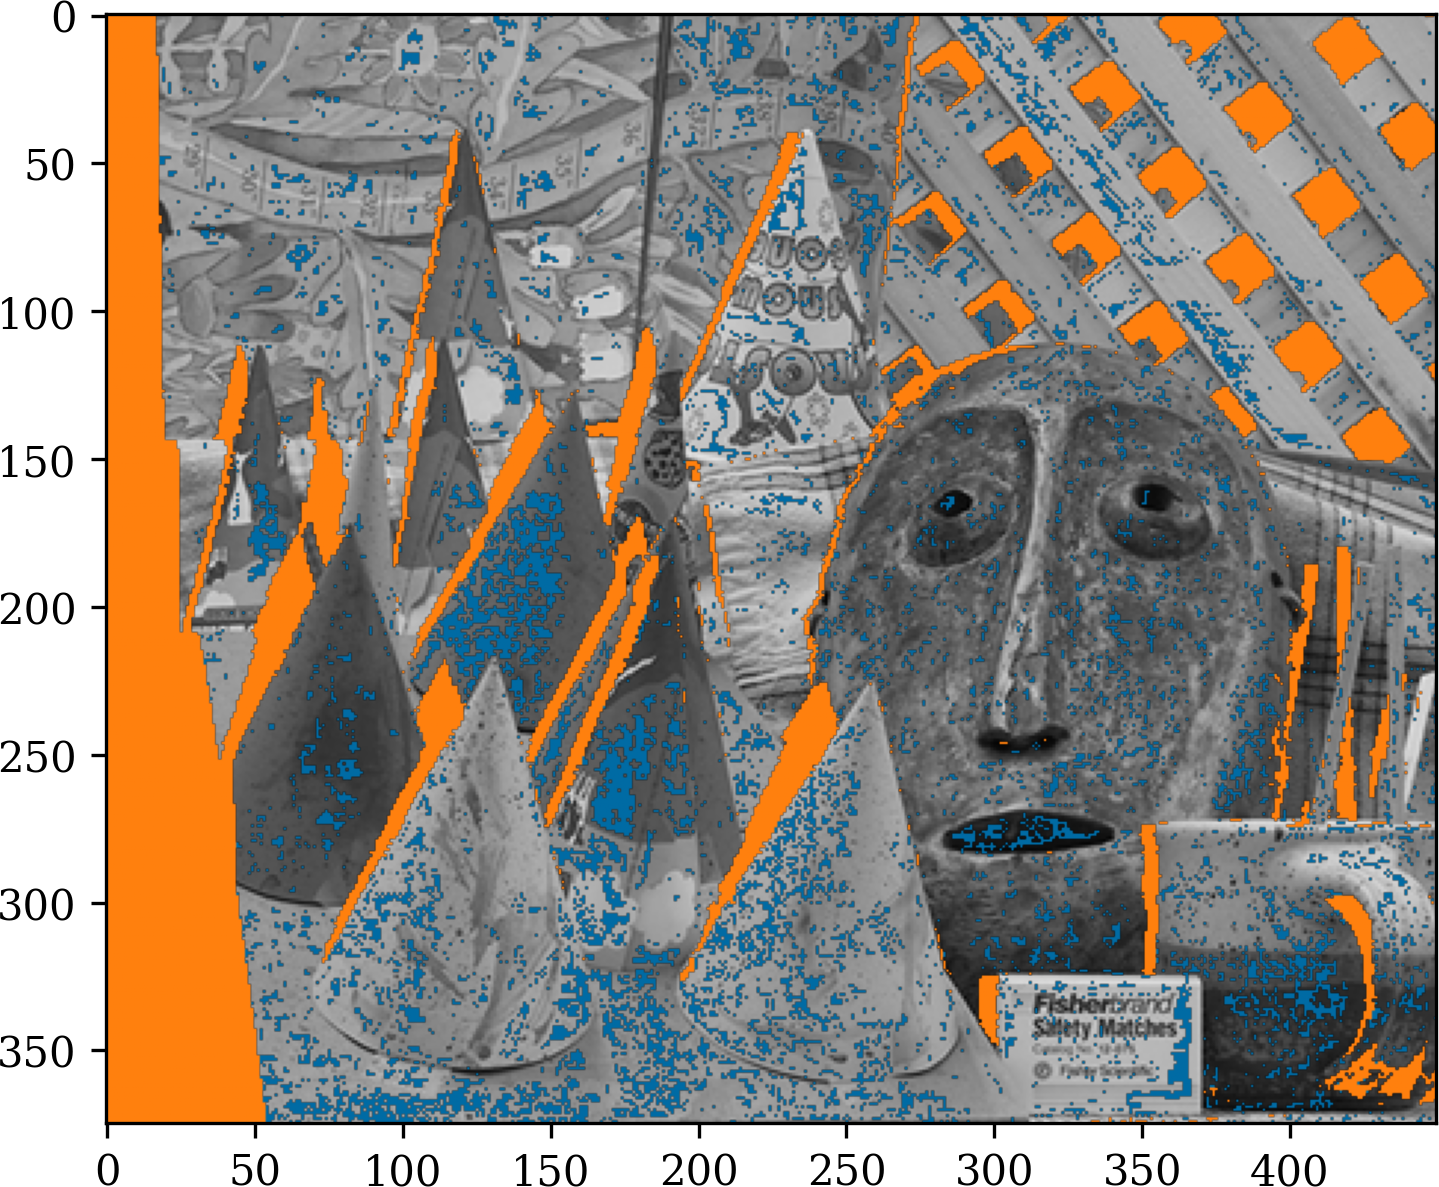
\includegraphics[width=\linewidth]{Images/Improvements_Pl=0.85.png}
        \caption{$\gamma=0.85,~\Delta s_\gamma=16.11\%$}
        \label{fig:improvements_b}
    \end{subfigure}\\
    \begin{subfigure}{0.48\linewidth}
        \centering
        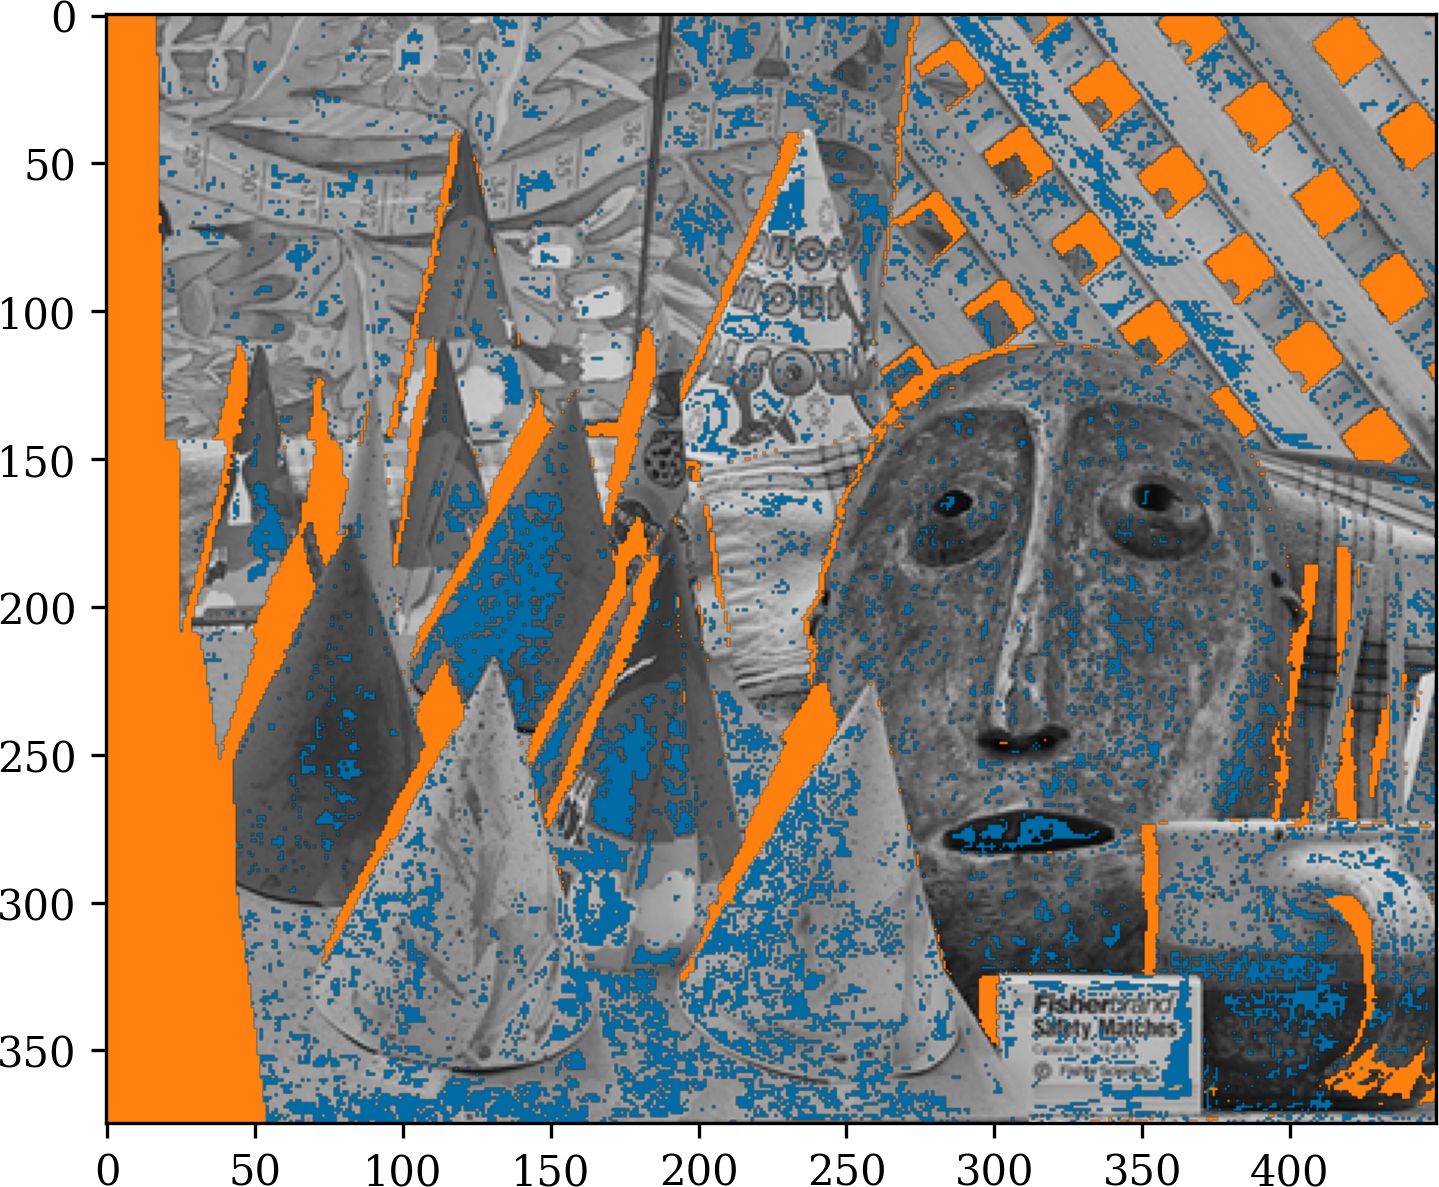
\includegraphics[width=\linewidth]{Images/Improvements_Pl=0.5.png}
        \caption{$\gamma=0.5,~\Delta s_\gamma=21.41\%$}
        \label{fig:improvements_c}
    \end{subfigure}
    \begin{subfigure}{0.48\linewidth}
        \centering
        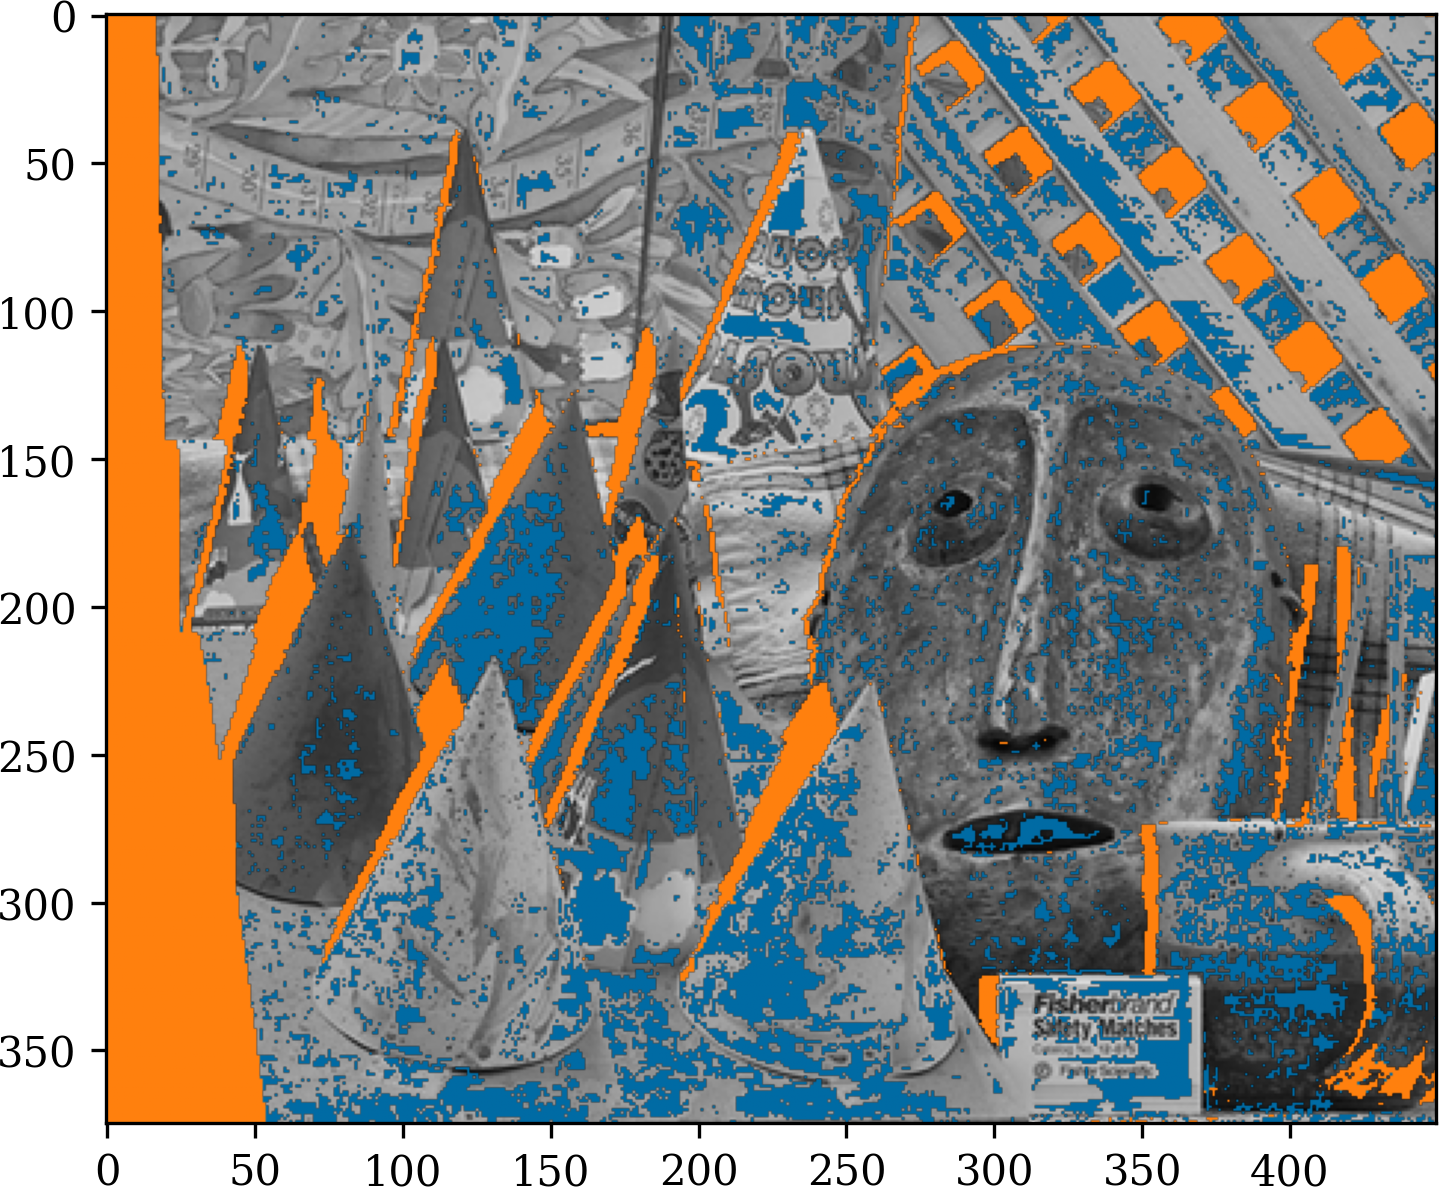
\includegraphics[width=\linewidth]{Images/Improvements_Pl=0.0.png}
        \caption{$\gamma=0,~\Delta s_\gamma=28.87\%$}
        \label{fig:improvements_d}
    \end{subfigure}
    \caption{Spatial disposition of potential improvements for different values of $\gamma$. Pixels with potential improvements appear in blue. Occluded pixels, for which a correct disparity does not exist, appear in orange. Grayscale left image is displayed on the background.}
    \label{fig:improvements}
\end{figure}

\section{Leveraging Confidence Envelopes for Potential Improvements}

Knowing the uncertainty, in our case represented as confidence envelopes, can provide valuable insights into potential matches. This section outlines observations suggesting that incorporating this information can enhance the performance of stereo-matching algorithms.

A common metric for evaluating stereo algorithm performance is the proportion of pixels $(row, col)$ for which the absolute difference between the true disparity and the predicted disparity is less than one pixel. This metric is used as we only consider integer disparities, but the ground truth disparity can be any real number in the disparity range. We thus consider a disparity to be ``correct'' if it is less than one pixel away from the true disparity. With this definition, there can be two ``correct'' disparities for every cost curve, which is inherent to the limited number of disparities one can consider. Let $d_{\mathrm{true}}(row, col)$ denote the true disparity and $\tilde{d}(row, col) = \arg \min_d \mathrm{SAD}(row, col, d)$ be the estimated disparity at pixel $(row, col)$. The score \( s \) is defined as:
\begin{equation}
    s = \frac{\#\{(row, col) \text{ such that } |d_{\mathrm{true}}(row, col) - \tilde{d}(row, col)| < 1\}}{\#\{(row, col)\}}\,.
\end{equation}

For a given confidence level $\gamma \in [0, 1]$ and a pixel $(row, col)$, we define the set of potential disparities $D_\gamma^{row, col}$ as:
\begin{equation}
    D_\gamma^{row, col} = \{d \mid \underline{\mathrm{SAD}}_\gamma(row, col, d) \leq \overline{\mathrm{SAD}}_\gamma(row, col, \tilde{d})\}\,.
\end{equation}

This set contains all disparities for which the lower estimate of $\mathrm{SAD}_\gamma$ at confidence level $\gamma$ is less than or equal to the upper estimate of $\mathrm{SAD}_\gamma$ at the predicted disparity $\tilde{d}$.

To evaluate if this set holds relevant information, we compute the optimal score \( s_\gamma^{\text{opt}} \) achievable using the set of possible disparities:
\begin{equation}
    s_\gamma^{\text{opt}} = \frac{\#\{(row, col) \mid \min_{d \in D_\gamma^{row, col}} |d_{\mathrm{true}}(row, col) - d| < 1\}}{\#\{(row, col)\}}\,.
\end{equation}

\todoroman{Inclure un schéma pour montrer ce qu'est $s_\gamma$}

We define the potential gain as \( \Delta s_\gamma = s_\gamma^{\text{opt}} - s \). Examples of optimal scores and potential gains for various $\gamma$ values are provided in Table \ref{tab:optimal_score}. We can see that while the potential gain for $\gamma = 0.9$ is low, it increases significantly for $\gamma$ values closer to $0$.

A pixel at position $(row, col)$ benefits from the method if:
\begin{equation}
    |d_{\mathrm{true}}(row, col) - \tilde{d}(row, col)| \geq 1 \quad \text{and} \quad \min_{d \in D_\gamma^{row, col}} |d_{\mathrm{true}}(row, col) - d| < 1
\end{equation}
In simpler terms, the disparity at a given position could be improved if it is currently not correct, and if a correct  disparity is in $D_\gamma^{row, col}$.

Figure \ref{fig:improvements} displays the spatial distribution of pixels that can benefit from this method. Pixels in occluded regions, \ie pixels only appearing in one of the two images, are highlighted in orange. Those pixels cannot be improved as no true disparity exists. Pixels where potential improvement can occur are shown in blue. Notably, these pixels are typically found in homogeneous areas where multiple disparities have low matching costs, as illustrated in Figure \ref{fig:montecarlo_gauss_200_150_large}. For those cost curves, there can exist a cost curve contained in the plausibility envelopes which would give a correct disparity as its minimum.

\begin{table}[ht]
\centering
\begin{tabular}{|c|c|c|c|c|}
\hline
\rowcolor[HTML]{C0C0C0} 
$s=52.87\%$                                & $\gamma=0.9$ & $\gamma=0.85$ & $\gamma=0.5$ & $\gamma=0$ \\ \hline
\cellcolor[HTML]{C0C0C0}$s_\gamma^{opt}$   & $56.92\%$    & $66.99\%$     & $74.28\%$    & $81.75\%$  \\ \hline
\cellcolor[HTML]{C0C0C0}$\Delta s_\gamma$ & $4.05\%$     & $16.11\%$     & $21.41\%$    & $28.87\%$  \\ \hline
\end{tabular}
\caption{Optimal score and potential gain for different plausibility $\gamma$. The potential gain is computed with regards to the usual score $s=52,87\%$.}\label{tab:optimal_score}
\end{table}


\pagebreak